\documentclass[10pt,a4paper]{article}
\usepackage[margin=0.72in]{geometry}
\usepackage{graphicx}
\usepackage{booktabs}
\usepackage{tabularx}
\usepackage{array}
\usepackage{float}
\usepackage{subcaption}
\usepackage{amsmath}
\usepackage{microtype}
\usepackage{enumitem}
\usepackage{xcolor}
\usepackage[hidelinks]{hyperref}
\usepackage{caption}
\captionsetup{font=small,labelfont=bf}
\setlength{\parskip}{0.42em}
\setlength{\parindent}{0pt}
\renewcommand{\arraystretch}{1.12}
\graphicspath{{../results_clean_split/final_artifacts/figures/}}
% Generated from results_clean_split by scripts/generate_report_data.py.
% Do not edit metric values manually.
\newcommand{\DatasetTotal}{9,114}
\newcommand{\DatasetTrain}{6,380}
\newcommand{\DatasetValidation}{1,368}
\newcommand{\DatasetTest}{1,366}
\newcommand{\DatasetTrainPct}{70.00}
\newcommand{\DatasetValidationPct}{15.01}
\newcommand{\DatasetTestPct}{14.99}
\newcommand{\HOneTrain}{3,083}
\newcommand{\HOneValidation}{661}
\newcommand{\HOneTest}{660}
\newcommand{\HTwoTrain}{1,634}
\newcommand{\HTwoValidation}{350}
\newcommand{\HTwoTest}{350}
\newcommand{\HThreeTrain}{573}
\newcommand{\HThreeValidation}{123}
\newcommand{\HThreeTest}{123}
\newcommand{\HFiveTrain}{573}
\newcommand{\HFiveValidation}{123}
\newcommand{\HFiveTest}{122}
\newcommand{\HSixTrain}{517}
\newcommand{\HSixValidation}{111}
\newcommand{\HSixTest}{111}
\newcommand{\ModelAParams}{2,553,349}
\newcommand{\ModelAAccuracy}{67.64}
\newcommand{\ModelATestLoss}{0.8360}
\newcommand{\ModelAPrecision}{0.6820}
\newcommand{\ModelARecall}{0.6360}
\newcommand{\ModelAFOne}{0.6254}
\newcommand{\ModelASizeMiB}{9.755}
\newcommand{\ModelASizeKiB}{9988.7}
\newcommand{\ModelATotalTime}{346.43}
\newcommand{\ModelAEpochTime}{17.32}
\newcommand{\ModelABestEpoch}{11}
\newcommand{\ModelAMACs}{62.325}
\newcommand{\ModelAFLOPs}{124.651}
\newcommand{\ModelAHTwoRecall}{0.1771}
\newcommand{\ModelBParams}{37,957}
\newcommand{\ModelBAccuracy}{70.57}
\newcommand{\ModelBTestLoss}{0.6755}
\newcommand{\ModelBPrecision}{0.7416}
\newcommand{\ModelBRecall}{0.6606}
\newcommand{\ModelBFOne}{0.6800}
\newcommand{\ModelBSizeMiB}{0.176}
\newcommand{\ModelBSizeKiB}{179.8}
\newcommand{\ModelBTotalTime}{253.80}
\newcommand{\ModelBEpochTime}{12.69}
\newcommand{\ModelBBestEpoch}{20}
\newcommand{\ModelBMACs}{7.263}
\newcommand{\ModelBFLOPs}{14.526}
\newcommand{\ModelBHTwoRecall}{0.2457}
\newcommand{\MobileParams}{2,230,277}
\newcommand{\MobileAccuracy}{86.09}
\newcommand{\MobileTestLoss}{0.3581}
\newcommand{\MobilePrecision}{0.8824}
\newcommand{\MobileRecall}{0.8825}
\newcommand{\MobileFOne}{0.8822}
\newcommand{\MobileSizeMiB}{8.740}
\newcommand{\MobileSizeKiB}{8949.4}
\newcommand{\MobileTotalTime}{753.41}
\newcommand{\MobileEpochTime}{37.66}
\newcommand{\MobileBestEpoch}{18}
\newcommand{\MobileMACs}{24.455}
\newcommand{\MobileFLOPs}{48.910}
\newcommand{\MobileHTwoRecall}{0.7600}
\newcommand{\ShuffleParams}{1,258,729}
\newcommand{\ShuffleAccuracy}{83.46}
\newcommand{\ShuffleTestLoss}{0.3968}
\newcommand{\ShufflePrecision}{0.8705}
\newcommand{\ShuffleRecall}{0.8519}
\newcommand{\ShuffleFOne}{0.8606}
\newcommand{\ShuffleSizeMiB}{4.966}
\newcommand{\ShuffleSizeKiB}{5084.7}
\newcommand{\ShuffleTotalTime}{482.69}
\newcommand{\ShuffleEpochTime}{24.13}
\newcommand{\ShuffleBestEpoch}{18}
\newcommand{\ShuffleMACs}{11.751}
\newcommand{\ShuffleFLOPs}{23.502}
\newcommand{\ShuffleHTwoRecall}{0.7457}
\newcommand{\SGDLearningRate}{0.010}
\newcommand{\SGDMomentum}{0.0}
\newcommand{\SGDBestVal}{66.01}
\newcommand{\SGDBestEpoch}{18}
\newcommand{\SGDFinalTrainLoss}{0.8961}
\newcommand{\SGDFinalValLoss}{0.8384}
\newcommand{\SGDTestLoss}{0.8358}
\newcommand{\SGDTestAccuracy}{65.67}
\newcommand{\SGDPrecision}{0.6705}
\newcommand{\SGDRecall}{0.5719}
\newcommand{\SGDFOne}{0.5844}
\newcommand{\SGDEpochTenVal}{63.45}
\newcommand{\MomentumLearningRate}{0.010}
\newcommand{\MomentumMomentum}{0.9}
\newcommand{\MomentumBestVal}{70.54}
\newcommand{\MomentumBestEpoch}{18}
\newcommand{\MomentumFinalTrainLoss}{0.7938}
\newcommand{\MomentumFinalValLoss}{0.7165}
\newcommand{\MomentumTestLoss}{0.7255}
\newcommand{\MomentumTestAccuracy}{68.81}
\newcommand{\MomentumPrecision}{0.6723}
\newcommand{\MomentumRecall}{0.6594}
\newcommand{\MomentumFOne}{0.6563}
\newcommand{\MomentumEpochTenVal}{68.42}
\newcommand{\AdamLearningRate}{0.001}
\newcommand{\AdamMomentum}{--}
\newcommand{\AdamBestVal}{73.25}
\newcommand{\AdamBestEpoch}{20}
\newcommand{\AdamFinalTrainLoss}{0.7510}
\newcommand{\AdamFinalValLoss}{0.6671}
\newcommand{\AdamTestLoss}{0.6755}
\newcommand{\AdamTestAccuracy}{70.57}
\newcommand{\AdamPrecision}{0.7416}
\newcommand{\AdamRecall}{0.6606}
\newcommand{\AdamFOne}{0.6800}
\newcommand{\AdamEpochTenVal}{70.54}
\newcommand{\ModelBAccuracyGainVsA}{2.93}
\newcommand{\ModelBParamReductionVsA}{98.51}
\newcommand{\ModelBParamFactorVsA}{67.27}
\newcommand{\ModelBMACReductionVsA}{88.35}
\newcommand{\MobileAccuracyGainVsB}{15.52}
\newcommand{\MobileParamFactorVsB}{58.76}
\newcommand{\MobileSizeFactorVsB}{49.79}
\newcommand{\MobileMACFactorVsB}{3.37}
\newcommand{\ShuffleAccuracyGainVsB}{12.88}
\newcommand{\ShuffleParamFactorVsB}{33.16}
\newcommand{\ShuffleSizeFactorVsB}{28.29}
\newcommand{\ShuffleMACFactorVsB}{1.62}


\newcommand{\dash}{\textemdash}
\newcolumntype{Y}{>{\raggedright\arraybackslash}X}

\begin{document}
\pagenumbering{roman}
\begin{titlepage}
\centering
{\Large University of Moratuwa\par}
\vspace{0.35cm}
{\large EN3150 - Pattern Recognition\par}
\vspace{1.0cm}
{\Huge\bfseries Assignment 03\par}
\vspace{0.25cm}
{\LARGE\bfseries Resource-Constrained CNN for Edge Image Classification\par}
\vspace{1.0cm}
{\Large\bfseries Group: Draco\par}
{\large\itshape Dealing with AI from the core\par}
\vspace{0.8cm}
\begin{tabular}{ll}
\textbf{GUNARATHNA K.T.M.B.} & 230203G\\
\textbf{JAYAWARDANA K.P.P.} & 230294H\\
\textbf{JITHMAL P.G.I.} & 230306B\\
\textbf{NIMADITH W.N.A.C.} & 230442L\\
\end{tabular}
\vfill
\textbf{Repository:}\\
\url{https://github.com/NavigatorPrime/CNN-Image-Classifier}\\[0.3cm]
\textbf{Canonical branch:}\\
\texttt{EN3150-A03-Final-Corrected-Report-v3}
\vfill
{\large October 2026\par}
\end{titlepage}

\tableofcontents
\clearpage
\pagenumbering{arabic}

\section{Introduction and Measurement Convention}
This work studies five-class DeFungi image classification under a strict custom-model parameter budget. Two custom CNNs are compared with fine-tuned MobileNetV2 and ShuffleNetV2 1.0x. The final conclusions use only the corrected leakage-free split and the clean-split Stage 2 experiment artifacts.

Every final metric in this PDF is injected from saved JSON, CSV, classification-report, training-history, checkpoint, or profiler artifacts by \texttt{scripts/generate\_report\_data.py}. No contaminated-split value is used. Computational cost uses one convention for an input of $1\times3\times64\times64$: Conv2d and Linear multiply-accumulate operations (MACs) are counted; BatchNorm, activations, pooling, residual additions, concatenation, channel shuffle, softmax, and data movement are excluded. FLOPs are reported as $2\times$ MACs. These are calculated operation counts, not device latency measurements.

\section{Task 1: Data Preparation}
\subsection{Corrected common split}
The UCI DeFungi data contain classes H1, H2, H3, H5, and H6. All packaged images are RGB and exactly $64\times64$ pixels. Images were grouped using both raw-file SHA-256 and decoded-pixel SHA-256 before deterministic class-aware allocation. All members of an identical-content group remain in one split.

\begin{table}[H]
\centering
\caption{Corrected leakage-free dataset split.}
\begin{tabular}{lrrrrrr}
\toprule
Split & H1 & H2 & H3 & H5 & H6 & Total\\
\midrule
Train & \HOneTrain & \HTwoTrain & \HThreeTrain & \HFiveTrain & \HSixTrain & \DatasetTrain\\
Validation & \HOneValidation & \HTwoValidation & \HThreeValidation & \HFiveValidation & \HSixValidation & \DatasetValidation\\
Test & \HOneTest & \HTwoTest & \HThreeTest & \HFiveTest & \HSixTest & \DatasetTest\\
\bottomrule
\end{tabular}
\end{table}

The split percentages are \DatasetTrainPct\%, \DatasetValidationPct\%, and \DatasetTestPct\%. The validator found 59 duplicate-content groups inside the dataset but zero raw-byte or decoded-pixel duplicate groups crossing train, validation, and test. The manifest and physical package contain the same \DatasetTotal\ images.

\begin{figure}[H]
\centering
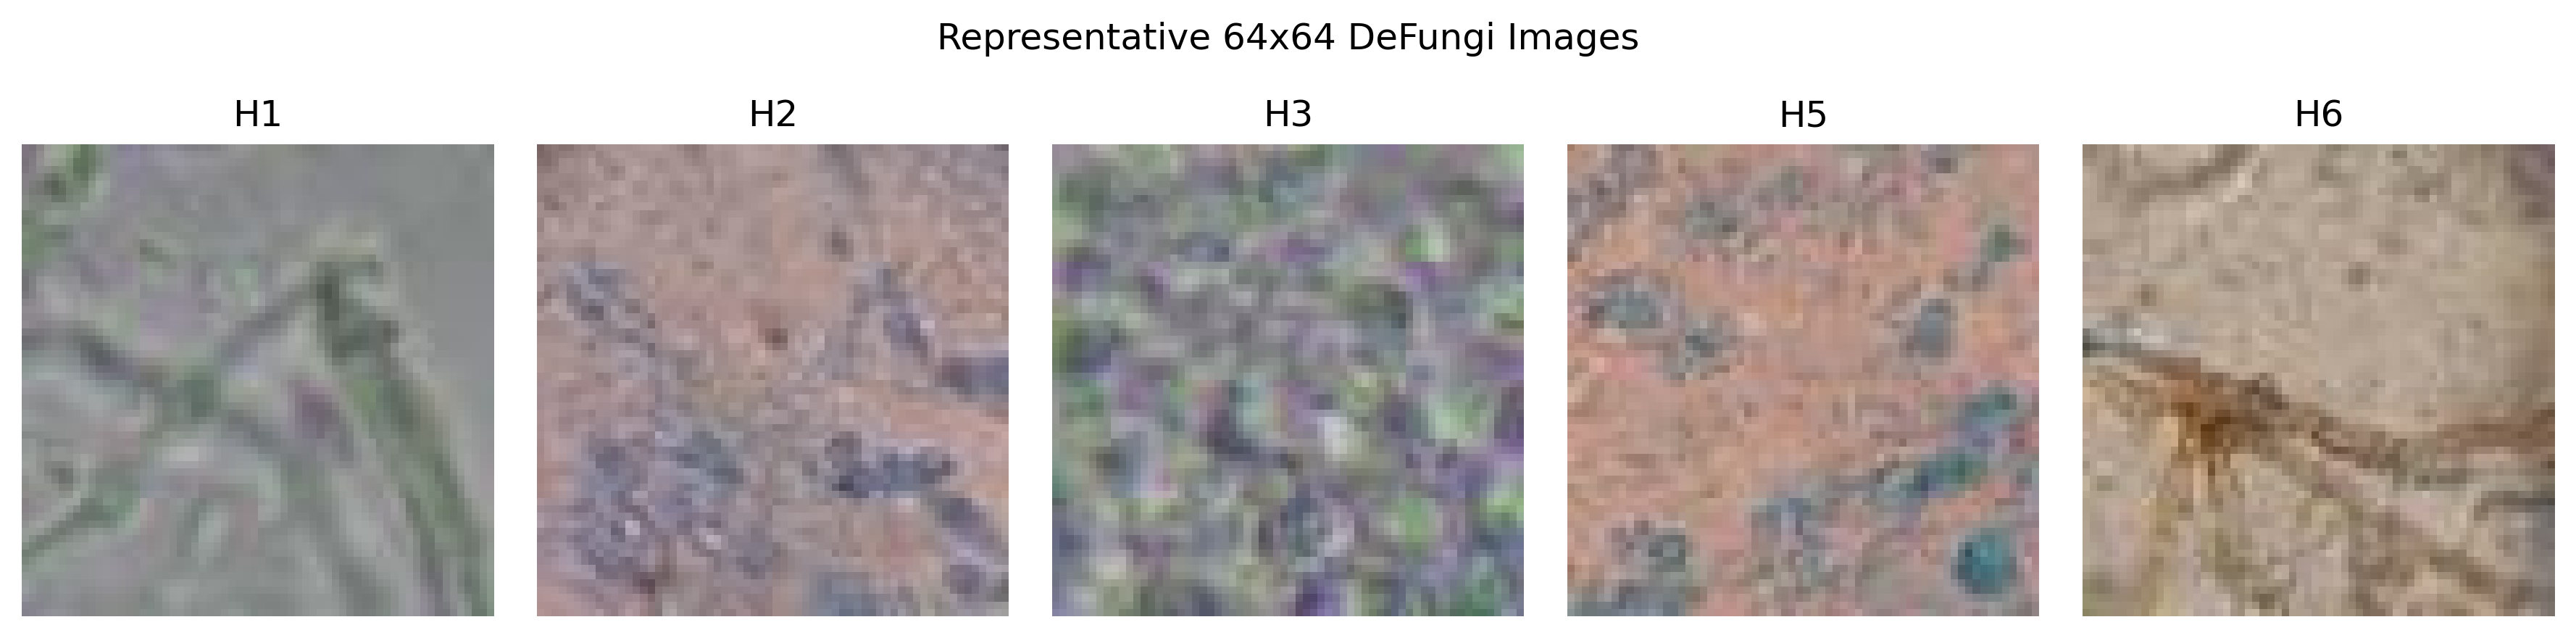
\includegraphics[width=0.92\linewidth]{task1/representative_samples.png}
\caption{Representative $64\times64$ RGB images from the corrected training split.}
\end{figure}

\begin{figure}[H]
\centering
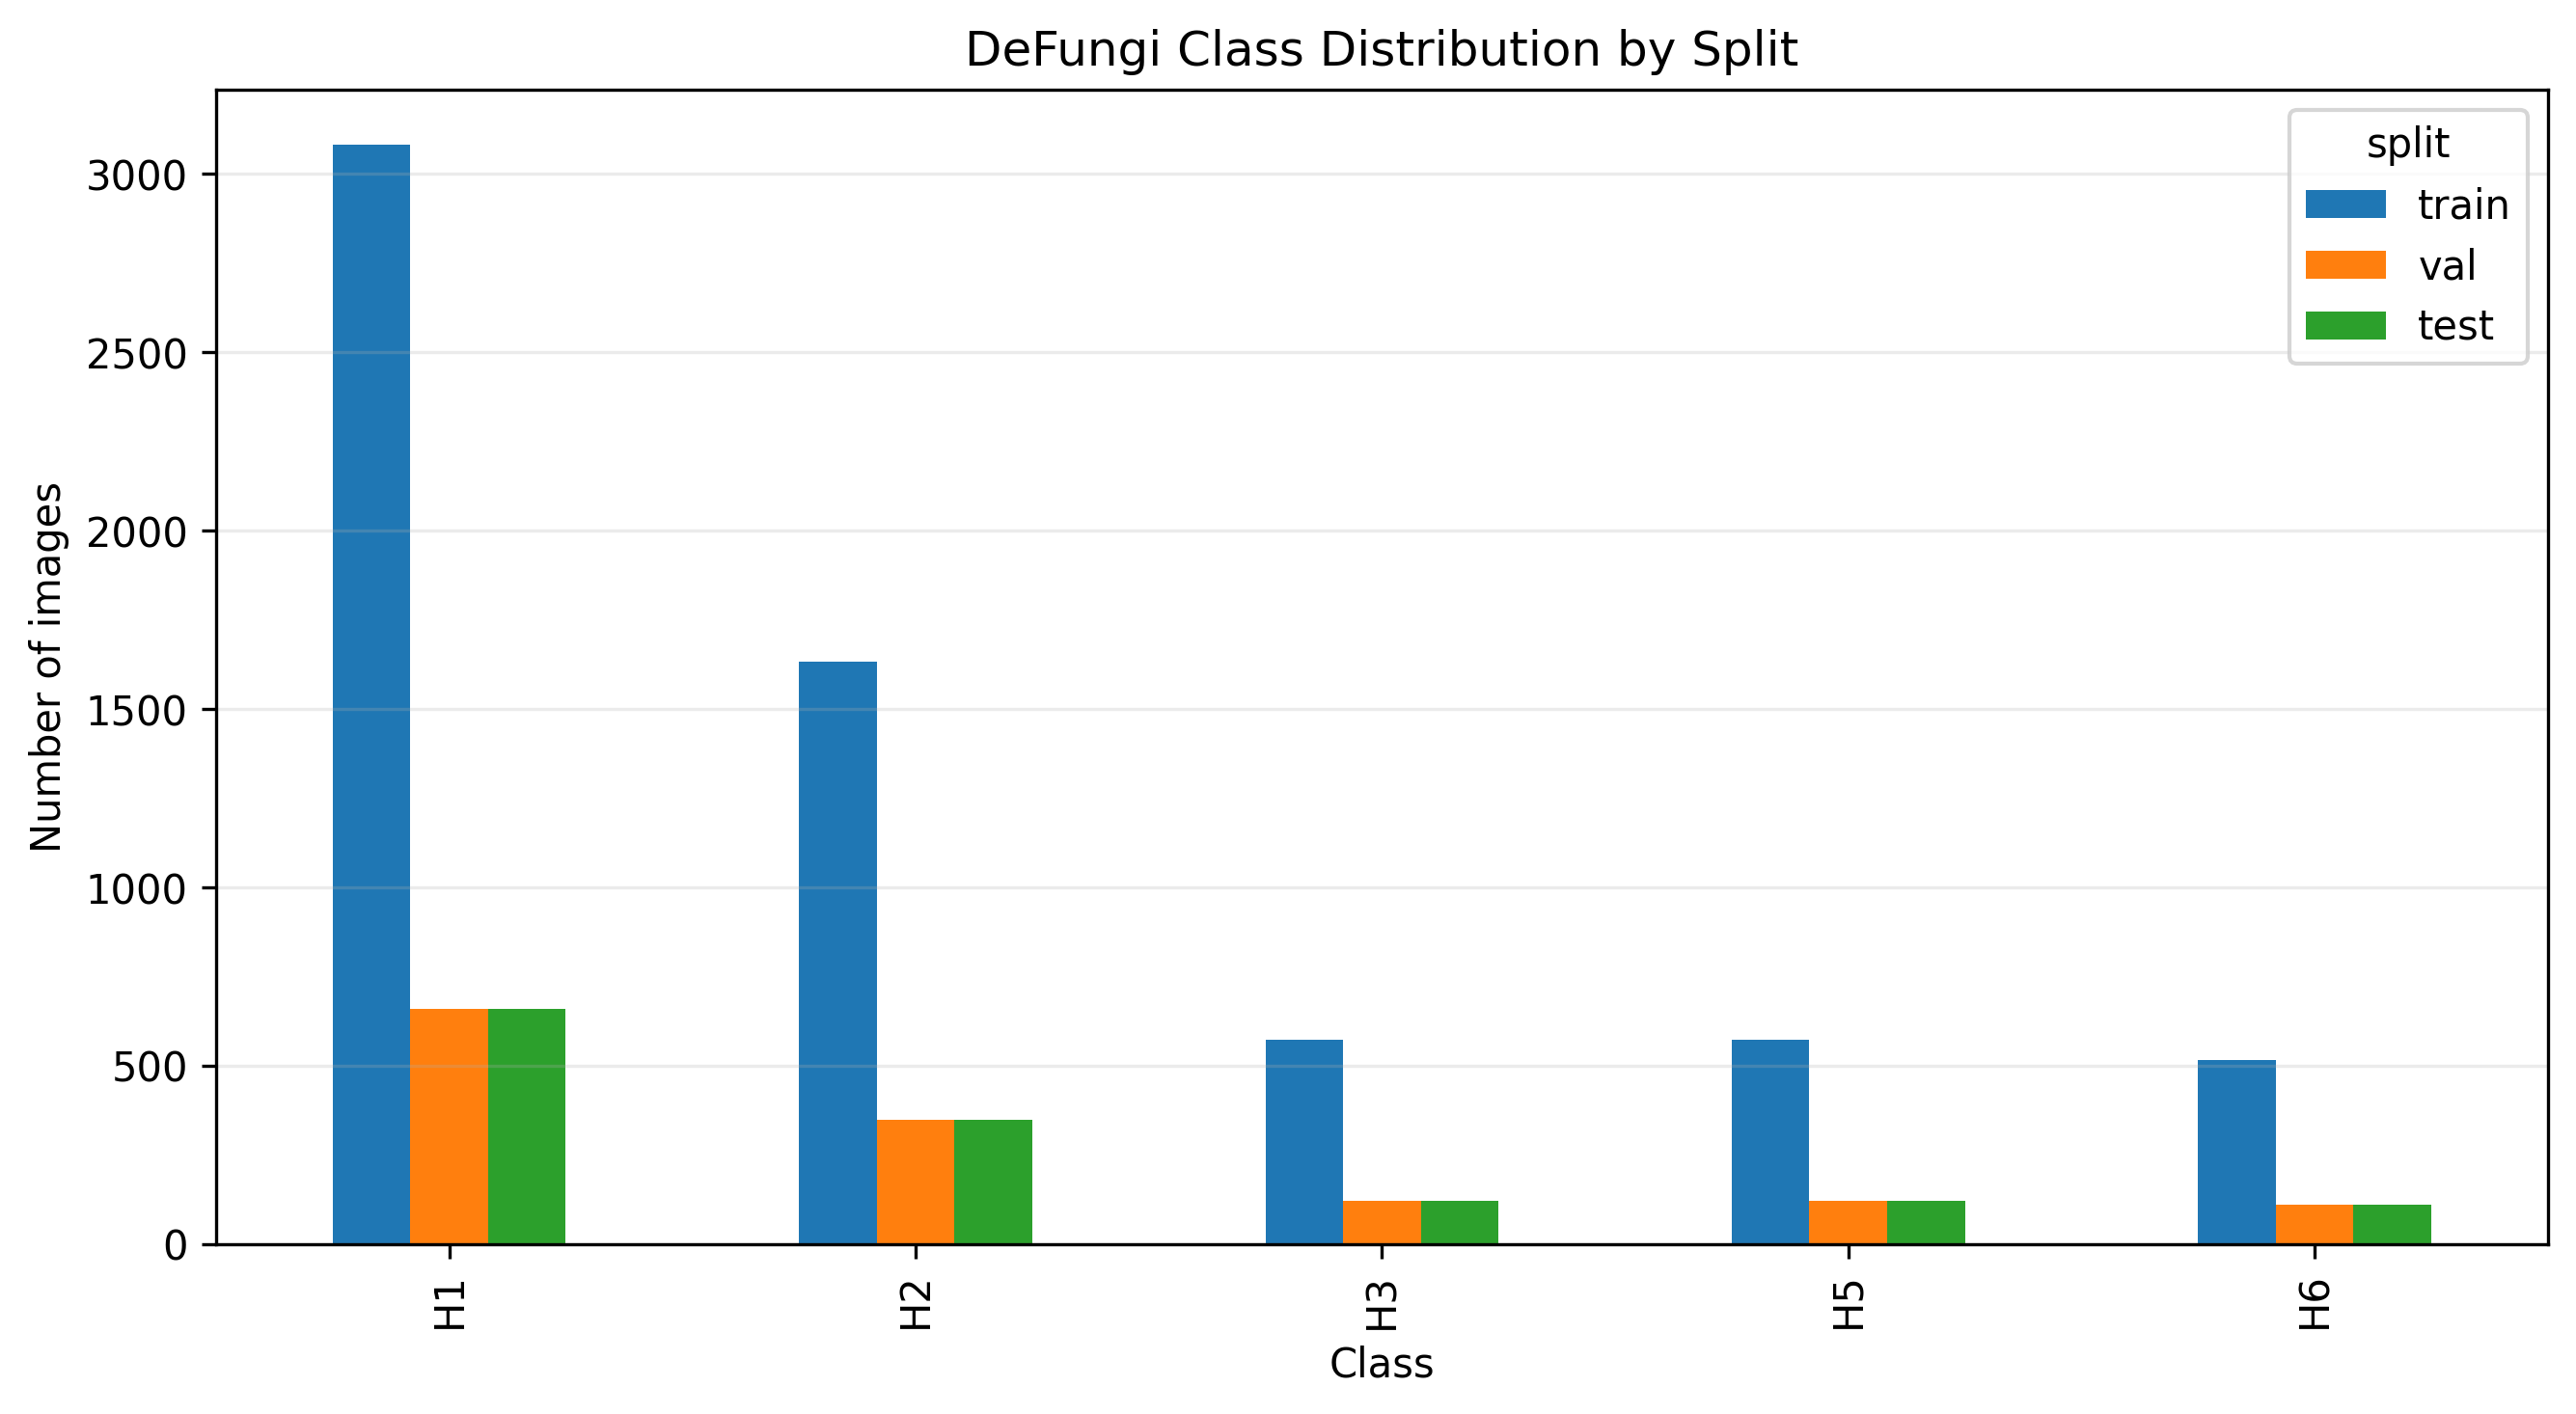
\includegraphics[width=0.78\linewidth]{task1/class_distribution.png}
\caption{Per-class distribution in the corrected common split. H1 and H2 dominate, so macro-averaged metrics are reported alongside accuracy.}
\end{figure}

Training preprocessing uses resize-to-$64\times64$, random horizontal and vertical flips, random rotation of $\pm15^\circ$, color jitter, tensor conversion, and ImageNet normalization. Validation and test preprocessing is deterministic and excludes augmentation. Seed 42 is used for reproducibility.

\section{Task 2: Custom Architecture Design}
\subsection{Model A: standard CNN}
Model A is a conventional four-block CNN. Each block uses standard $3\times3$ convolution, BatchNorm, ReLU, and $2\times2$ max pooling. The exact code-derived architecture is shown below.

\begin{table}[H]
\centering
\scriptsize
\caption{Model A architecture. ReLU, pooling, flattening, and dropout have no trainable parameters.}
\resizebox{\textwidth}{!}{%
\begin{tabular}{lllllllrr}
\toprule
Stage & Layer sequence & Input & Output filters/units & Kernel & Stride/padding & Output shape & Conv/FC & BN\\
\midrule
Block 1 & Conv2D, BN, ReLU, MaxPool & $3\times64\times64$ & 32 & $3\times3$; pool $2\times2$ & $1/1$; pool 2 & $32\times32\times32$ & 896 & 64\\
Block 2 & Conv2D, BN, ReLU, MaxPool & $32\times32\times32$ & 64 & $3\times3$; pool $2\times2$ & $1/1$; pool 2 & $64\times16\times16$ & 18,496 & 128\\
Block 3 & Conv2D, BN, ReLU, MaxPool & $64\times16\times16$ & 128 & $3\times3$; pool $2\times2$ & $1/1$; pool 2 & $128\times8\times8$ & 73,856 & 256\\
Block 4 & Conv2D, BN, ReLU, MaxPool & $128\times8\times8$ & 256 & $3\times3$; pool $2\times2$ & $1/1$; pool 2 & $256\times4\times4$ & 295,168 & 512\\
Flatten & Flatten & $256\times4\times4$ & 4096 & \dash & \dash & 4096 & 0 & 0\\
FC1 & Linear, ReLU, Dropout(0.5) & 4096 & 512 & \dash & \dash & 512 & 2,097,664 & 0\\
FC2 & Linear, ReLU, Dropout(0.3) & 512 & 128 & \dash & \dash & 128 & 65,664 & 0\\
Output & Linear logits & 128 & 5 & \dash & \dash & 5 & 645 & 0\\
\bottomrule
\end{tabular}}
\end{table}

For a biased Conv2D layer,
\[
P_{\mathrm{conv}}=(K_hK_wC_{\mathrm{in}}C_{\mathrm{out}})+C_{\mathrm{out}},
\]
and trainable BatchNorm contributes $2C_{\mathrm{out}}$ parameters (scale and shift). For example, Block 1 has $(3\cdot3\cdot3\cdot32)+32=896$ convolution parameters and $2\cdot32=64$ BatchNorm parameters. The four blocks total 389,376 parameters. The classifier contributes
\[
(4096\cdot512+512)+(512\cdot128+128)+(128\cdot5+5)=2,163,973.
\]
Therefore the verified total is $389,376+2,163,973=\mathbf{\ModelAParams}$ trainable parameters.

Model A uses ReLU after each convolutional BatchNorm and after the first two fully connected layers. ReLU is a simple threshold operation, so it avoids the exponential evaluations used by sigmoid and tanh. This is generally favorable for hardware implementation, but no target-device latency is claimed.

\subsection{Model B: depthwise-separable CNN}
Model B uses one standard convolutional stem followed by six depthwise-separable blocks, global average pooling (GAP), dropout, and a linear classifier. Each block applies depthwise Conv2D, BatchNorm, ReLU6, pointwise Conv2D, BatchNorm, and ReLU6.

\begin{table}[H]
\centering
\scriptsize
\caption{Model B architecture generated from the implementation. Block parameter totals include both convolutions and both BatchNorm layers.}
\resizebox{\textwidth}{!}{%
\begin{tabular}{llllllllrr}
\toprule
Stage & Input $C$ & DW $C$ & Groups & Kernel & Stride/pad & PW out & Output shape & Parameters & Activation\\
\midrule
Stem & 3 & \dash & 1 & $3\times3$ & $1/1$ & 16 & $16\times64\times64$ & 464 & ReLU6\\
DS Block 1 & 16 & 16 & 16 & $3\times3$ DW, $1\times1$ PW & $2/1$ & 32 & $32\times32\times32$ & 752 & ReLU6 $\times2$\\
DS Block 2 & 32 & 32 & 32 & $3\times3$ DW, $1\times1$ PW & $1/1$ & 32 & $32\times32\times32$ & 1,440 & ReLU6 $\times2$\\
DS Block 3 & 32 & 32 & 32 & $3\times3$ DW, $1\times1$ PW & $2/1$ & 64 & $64\times16\times16$ & 2,528 & ReLU6 $\times2$\\
DS Block 4 & 64 & 64 & 64 & $3\times3$ DW, $1\times1$ PW & $1/1$ & 64 & $64\times16\times16$ & 4,928 & ReLU6 $\times2$\\
DS Block 5 & 64 & 64 & 64 & $3\times3$ DW, $1\times1$ PW & $2/1$ & 128 & $128\times8\times8$ & 9,152 & ReLU6 $\times2$\\
DS Block 6 & 128 & 128 & 128 & $3\times3$ DW, $1\times1$ PW & $1/1$ & 128 & $128\times8\times8$ & 18,048 & ReLU6 $\times2$\\
GAP & 128 & \dash & \dash & global & \dash & 128 & $128\times1\times1$ & 0 & \dash\\
Dropout & 128 & \dash & \dash & \dash & \dash & 128 & 128 & 0 & \dash\\
Classifier & 128 & \dash & \dash & \dash & \dash & 5 & 5 logits & 645 & Linear\\
\bottomrule
\end{tabular}}
\end{table}

The depthwise and pointwise convolution parameter formulas are
\[
P_{\mathrm{DW}}=K_hK_wC_{\mathrm{in}} \quad\text{and}\quad
P_{\mathrm{PW}}=C_{\mathrm{in}}C_{\mathrm{out}},
\]
because both use \texttt{bias=False}. Their BatchNorm terms are $2C_{\mathrm{in}}$ and $2C_{\mathrm{out}}$. Thus a complete block has
\[
P_{\mathrm{block}}=9C_{\mathrm{in}}+2C_{\mathrm{in}}+C_{\mathrm{in}}C_{\mathrm{out}}+2C_{\mathrm{out}}.
\]
For Block 1 this is $144+32+512+64=752$. For Block 2, whose output width is also 32, it is $288+64+1024+64=1,440$. The stem has $3\cdot16\cdot9+2\cdot16=464$ parameters and the classifier has $128\cdot5+5=645$. Summing every row gives:
\[
\boxed{\text{Model B trainable parameters}=\ModelBParams<100,000.}
\]

For convolutional arithmetic alone, the depthwise-separable to standard-convolution ratio is $1/C_{\mathrm{out}}+1/9$. It is 14.24\% for the 16-to-32 and 32-to-32 blocks, and decreases for 64- and 128-output blocks. This comparison excludes BatchNorm and activation work, consistent with the project MAC convention.

Model B uses ReLU6 after the stem and after both convolution stages in every separable block. ReLU6 adds an upper clamp to ReLU's lower threshold; both remain simple piecewise-linear operations without exponential functions. The final classifier is strictly linear and produces five logits directly for \texttt{CrossEntropyLoss}; no output ReLU6 or softmax layer is applied in the model.

\section{Task 3: Optimizer Selection and Tuning}
\subsection{Controlled comparison}
The three Model B trials used the exact same corrected split, initial-state hash, seed 42, batch size 32, augmentation, cross-entropy loss, weight decay $10^{-4}$, and highest-validation-accuracy checkpoint rule. Each ran for 20 epochs. All used \texttt{ReduceLROnPlateau} on validation loss with factor 0.5 and patience 4; the learning rate did not reduce during these runs.

\begin{table}[H]
\centering
\scriptsize
\caption{Controlled clean-split optimizer comparison.}
\resizebox{\textwidth}{!}{%
\begin{tabular}{lrrrrrrrr}
\toprule
Optimizer & LR & Momentum & Best val. acc. & Epoch & Final train loss & Final val. loss & Test loss & Test acc.\\
\midrule
Standard SGD & \SGDLearningRate & \SGDMomentum & \SGDBestVal\% & \SGDBestEpoch & \SGDFinalTrainLoss & \SGDFinalValLoss & \SGDTestLoss & \SGDTestAccuracy\%\\
SGD + Momentum & \MomentumLearningRate & \MomentumMomentum & \MomentumBestVal\% & \MomentumBestEpoch & \MomentumFinalTrainLoss & \MomentumFinalValLoss & \MomentumTestLoss & \MomentumTestAccuracy\%\\
Adam & \AdamLearningRate & \AdamMomentum & \textbf{\AdamBestVal\%} & \AdamBestEpoch & \textbf{\AdamFinalTrainLoss} & \textbf{\AdamFinalValLoss} & \textbf{\AdamTestLoss} & \textbf{\AdamTestAccuracy\%}\\
\bottomrule
\end{tabular}}
\end{table}

\begin{figure}[H]
\centering
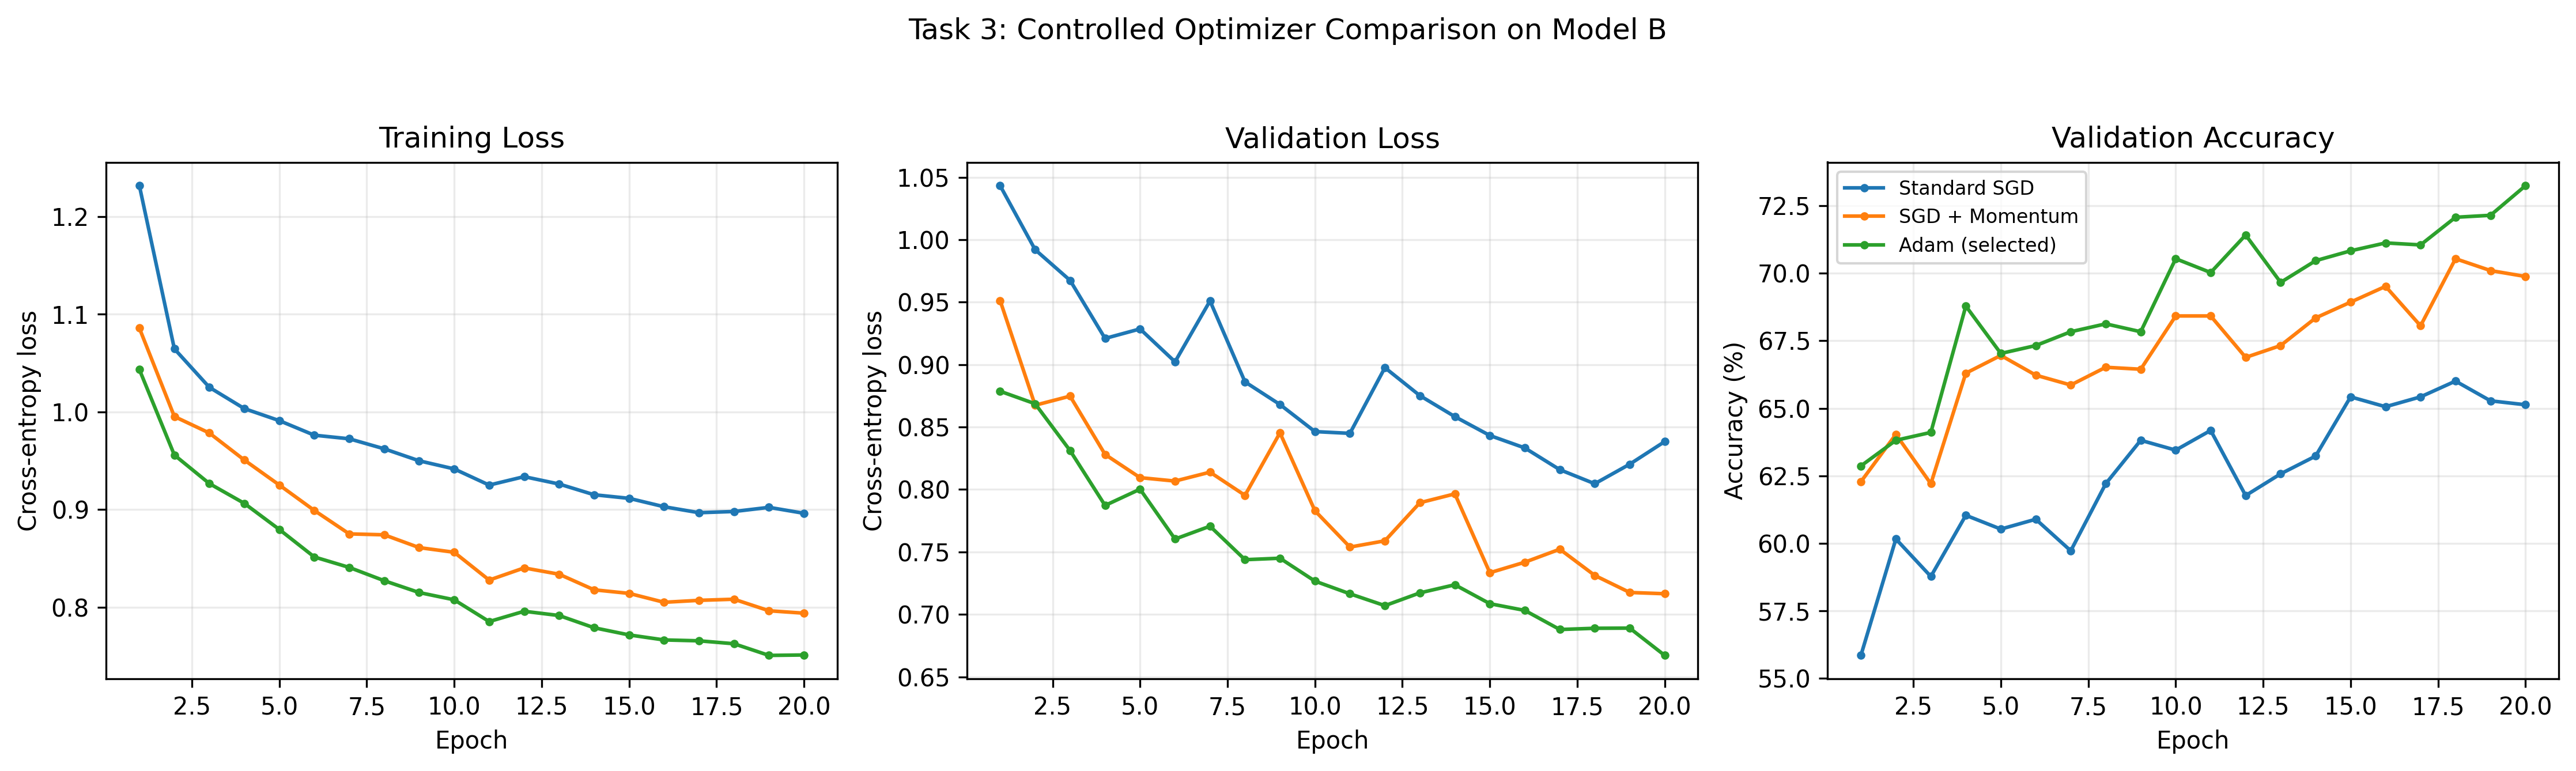
\includegraphics[width=\linewidth]{task3/optimizer_comparison_curves.png}
\caption{Training loss, validation loss, and validation accuracy for the controlled 20-epoch optimizer comparison.}
\end{figure}

\subsection{Momentum effect}
Momentum accumulates a velocity in directions supported by successive gradients:
\[
v_t=\mu v_{t-1}+g_t,\qquad \theta_{t+1}=\theta_t-\eta v_t.
\]
This can reduce oscillation and accelerate progress along consistent directions. The corrected curves support that interpretation: by epoch 10, SGD with momentum reached \MomentumEpochTenVal\% validation accuracy compared with \SGDEpochTenVal\% for plain SGD. Momentum also achieved a higher best validation accuracy (\MomentumBestVal\% versus \SGDBestVal\%), lower final validation loss (\MomentumFinalValLoss{} versus \SGDFinalValLoss), and higher test accuracy (\MomentumTestAccuracy\% versus \SGDTestAccuracy\%).

\subsection{Why Adam and learning rate 0.001 were selected}
Adam was selected because it produced the strongest controlled result within the fixed 20-epoch budget: \AdamBestVal\% best validation accuracy, \AdamTestAccuracy\% test accuracy, and macro F1 \AdamFOne. These exceed both plain SGD and SGD with momentum. Its curves also show useful progress throughout training, reaching \AdamEpochTenVal\% validation accuracy by epoch 10 and the best checkpoint at epoch \AdamBestEpoch. Adam combines momentum-like first-moment estimation with second-moment scaling, adapting the effective step size for each parameter. This reduces the amount of manual gradient-scale tuning required by plain SGD, while the conclusion here remains grounded in the measured comparison rather than optimizer theory alone.

The base learning rate 0.001 is a standard practical starting point for Adam and is smaller than the 0.01 used for the SGD variants. Because Adam rescales updates with first- and second-moment estimates, this smaller base rate helps avoid excessively large parameter updates while still permitting progress. In the corrected experiment it produced stable decreasing losses and the best validation result within 20 epochs. The plateau scheduler was configured but did not need to lower the rate, so all recorded Adam epochs used 0.001.

\section{Task 4: Custom Model Training and Evaluation}
Both canonical custom-model runs used the corrected split for 20 epochs and evaluated the test set only after restoring the selected checkpoint.

\begin{figure}[H]
\centering
\begin{subfigure}{0.49\linewidth}\centering
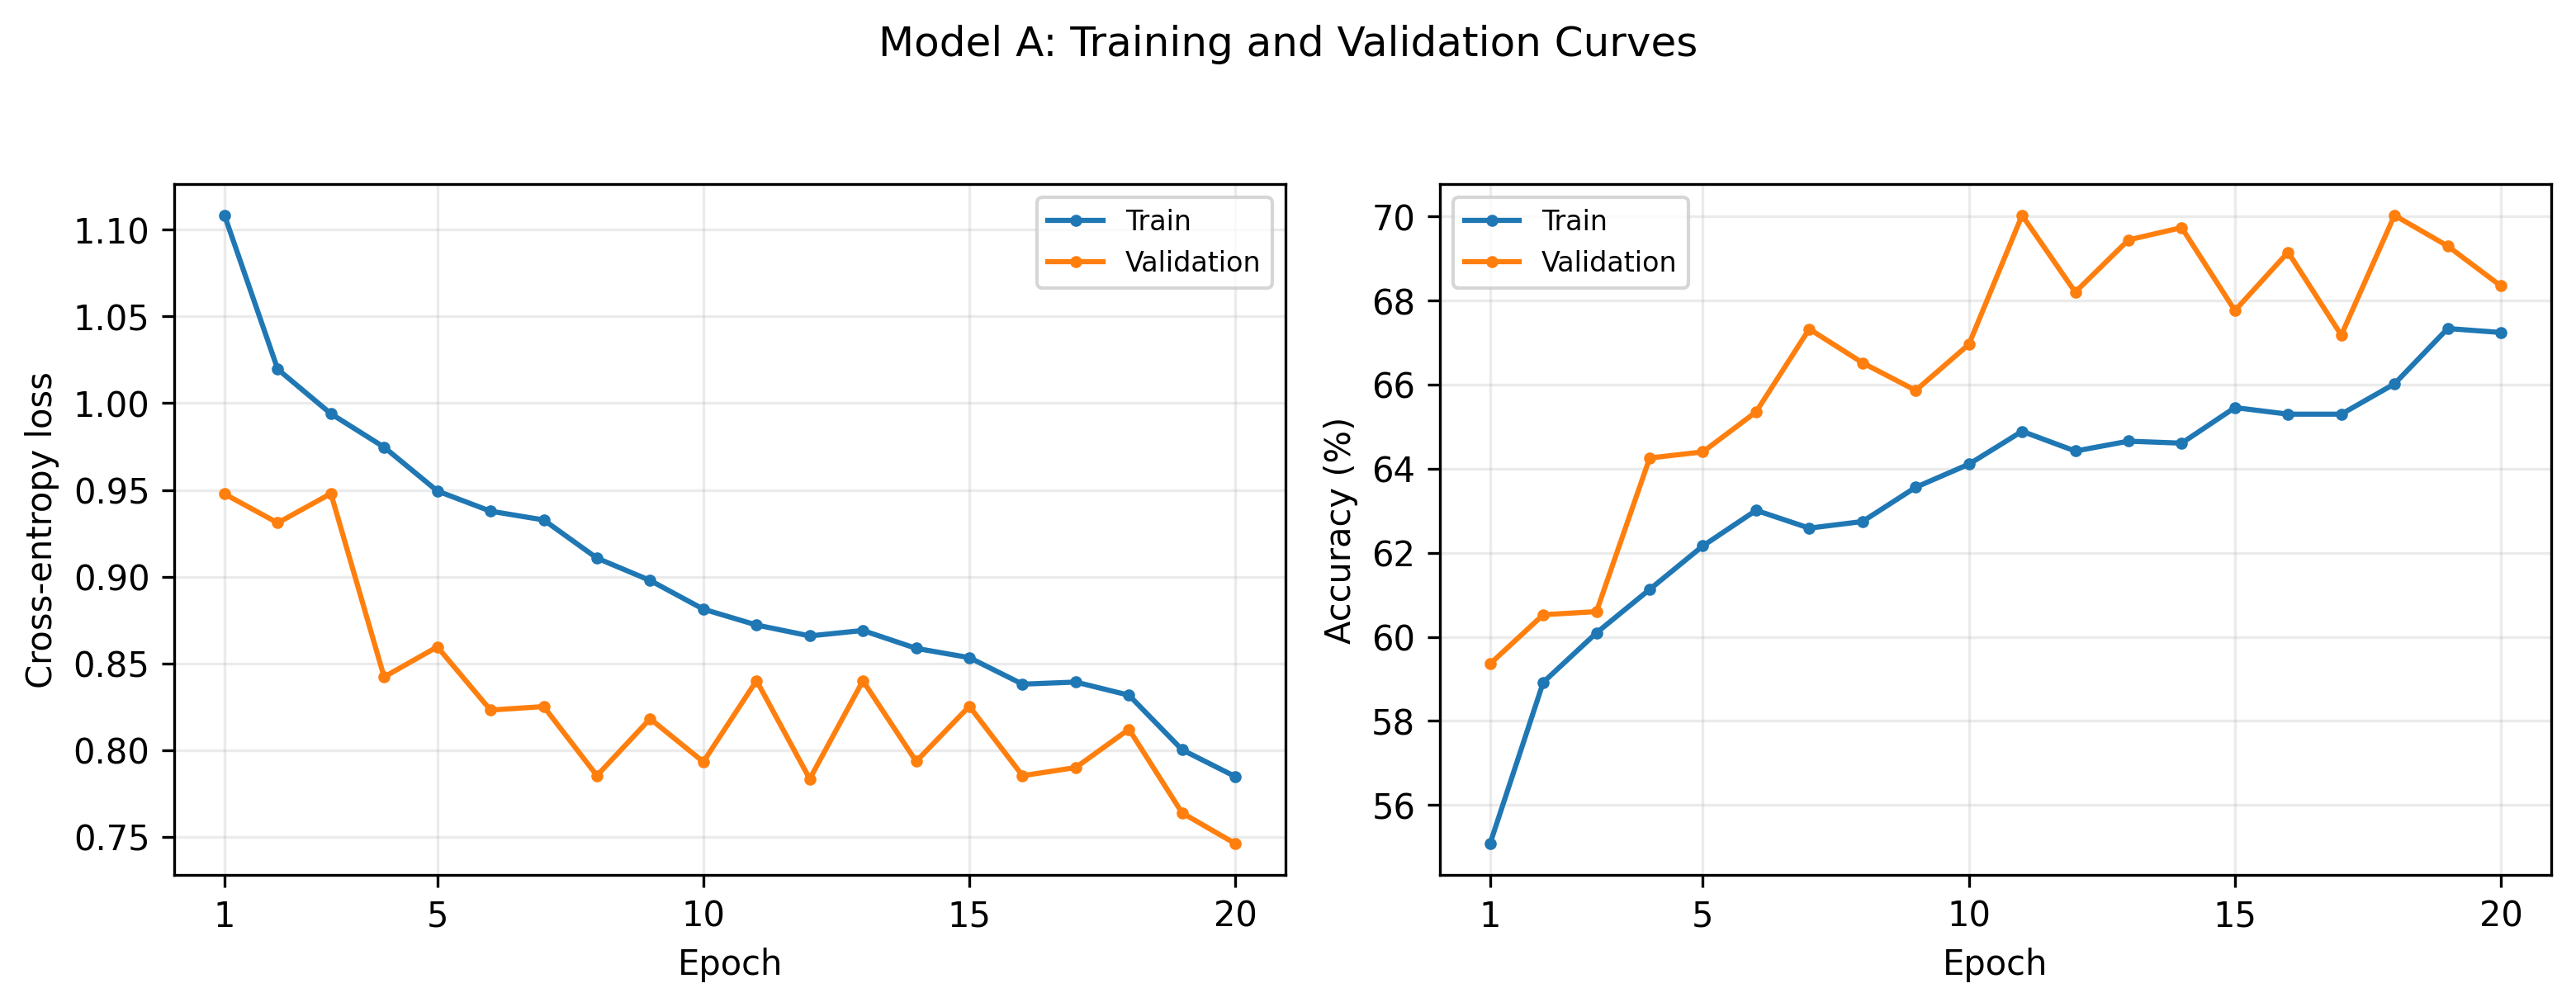
\includegraphics[width=\linewidth]{task4/model_a_training_curves.png}
\caption{Model A.}
\end{subfigure}\hfill
\begin{subfigure}{0.49\linewidth}\centering
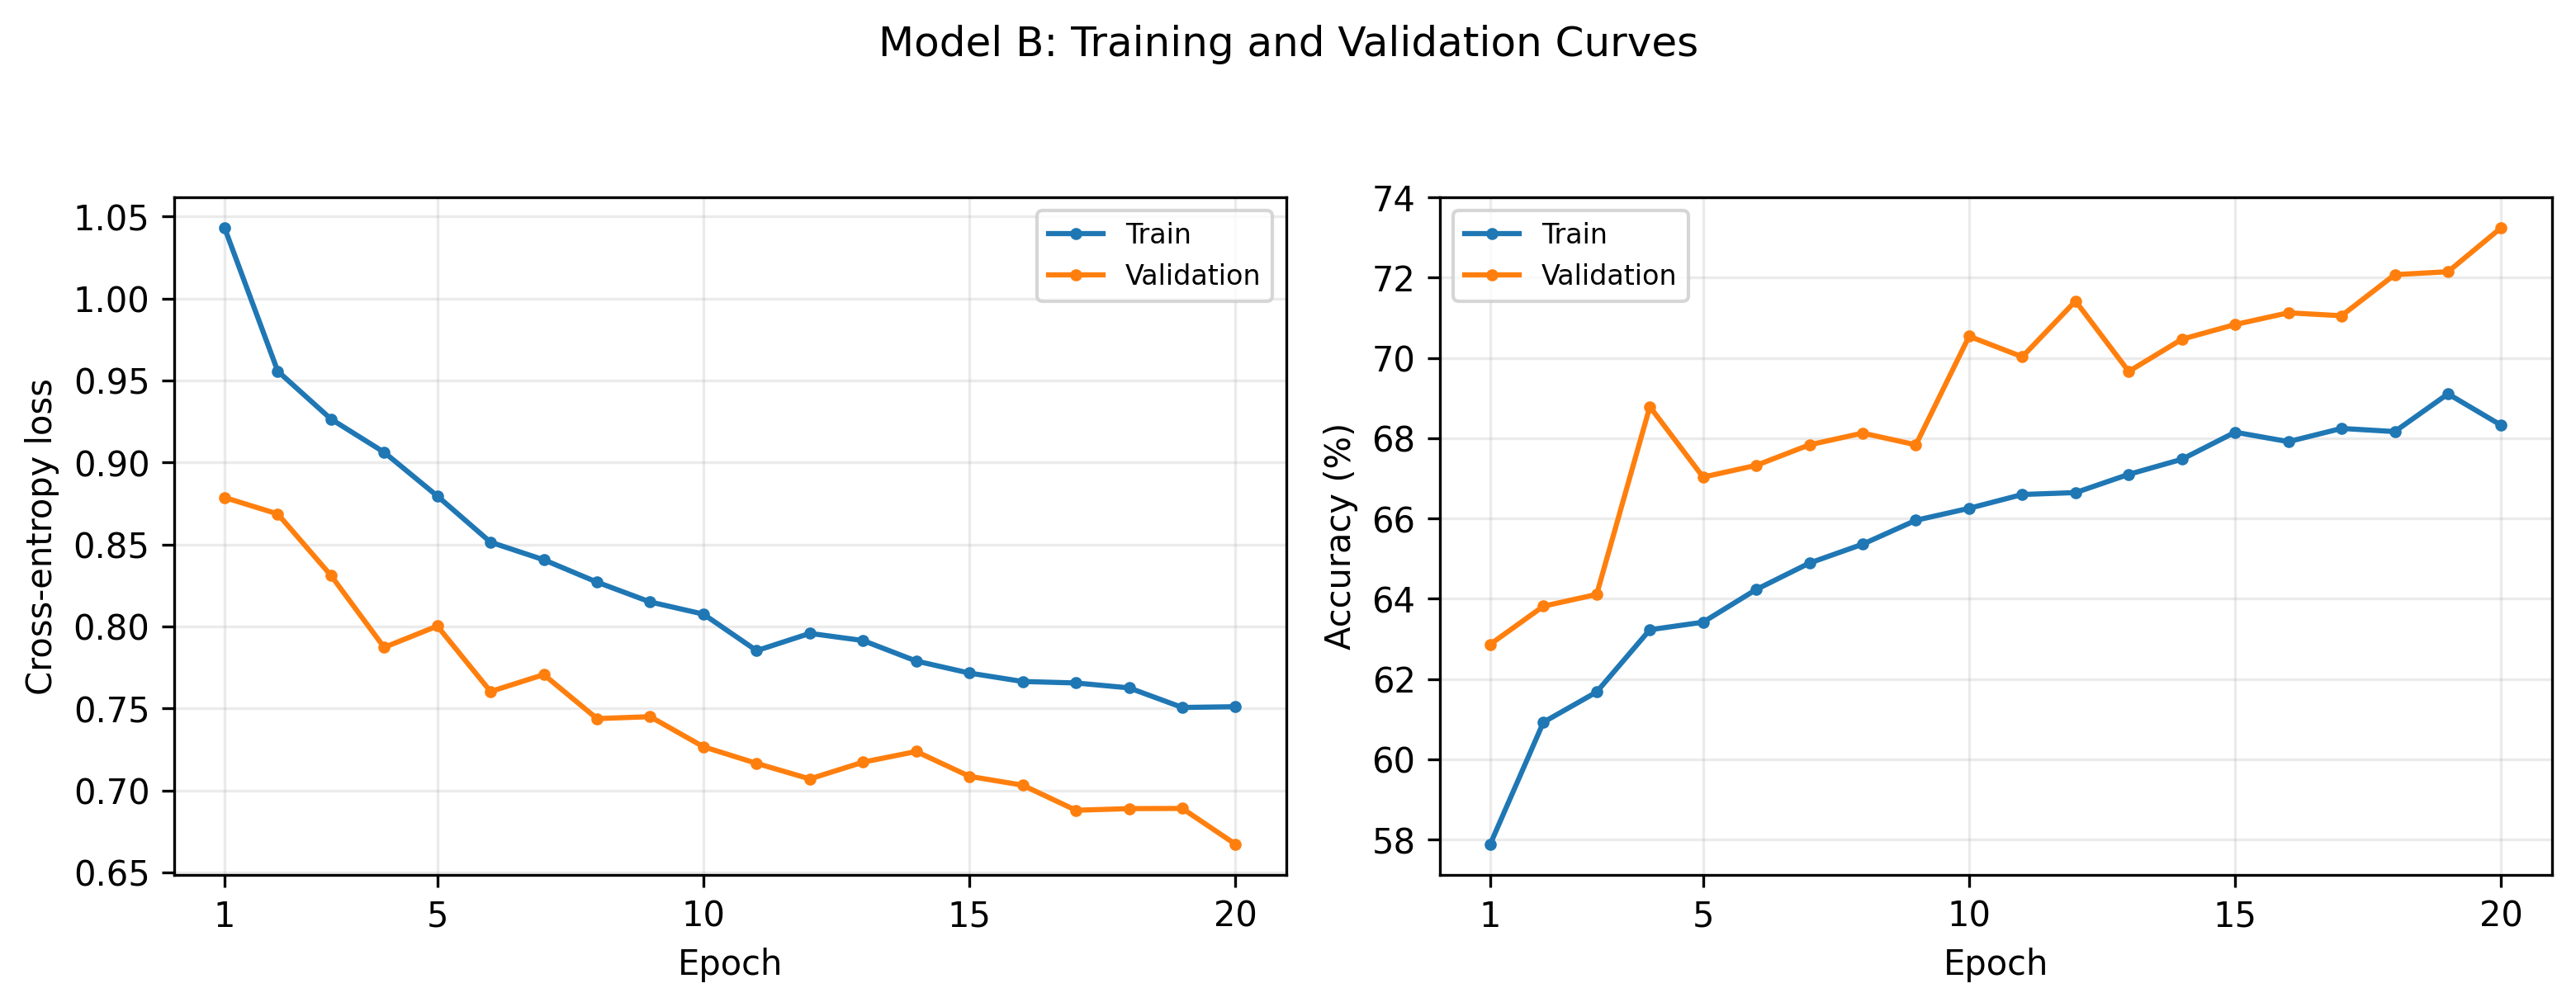
\includegraphics[width=\linewidth]{task4/model_b_training_curves.png}
\caption{Model B.}
\end{subfigure}
\caption{Training and validation loss and accuracy for the two custom models.}
\end{figure}

\begin{figure}[H]
\centering
\begin{subfigure}{0.49\linewidth}\centering
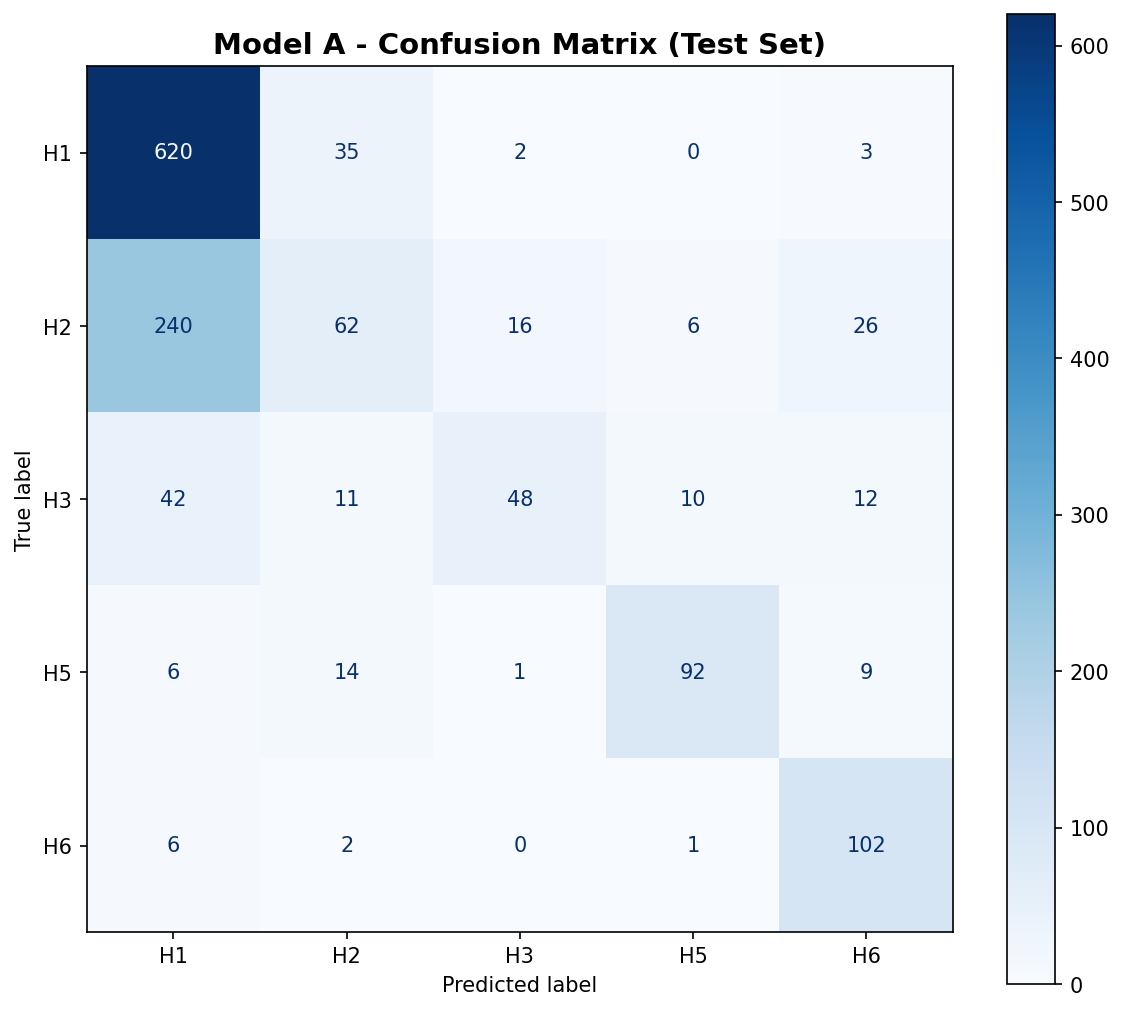
\includegraphics[width=\linewidth]{task4/model_a_confusion_matrix.png}
\caption{Model A.}
\end{subfigure}\hfill
\begin{subfigure}{0.49\linewidth}\centering
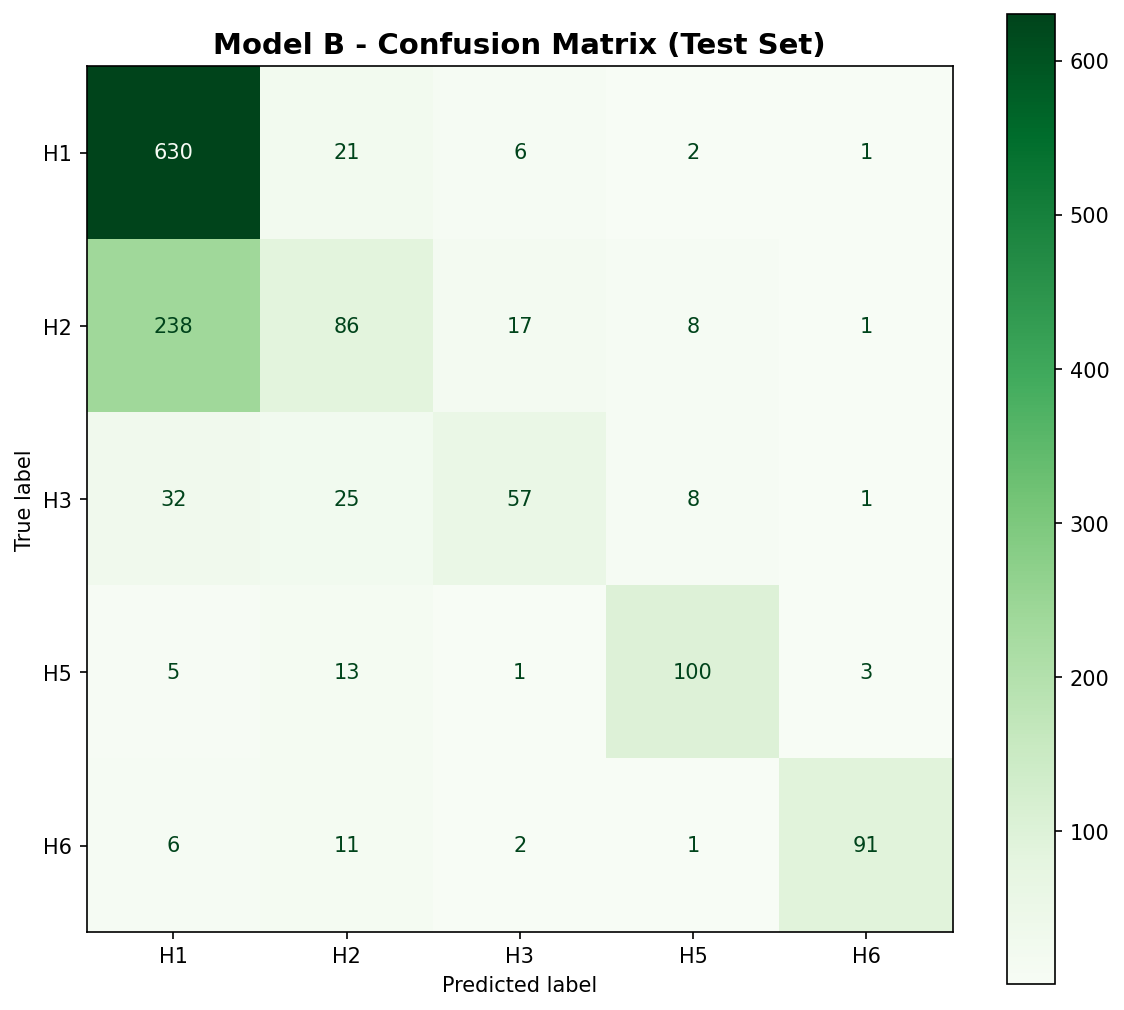
\includegraphics[width=\linewidth]{task4/model_b_confusion_matrix.png}
\caption{Model B.}
\end{subfigure}
\caption{Corrected test-set confusion matrices; each totals \DatasetTest\ images.}
\end{figure}

\begin{table}[H]
\centering
\scriptsize
\caption{Canonical clean-split custom-model results. Checkpoint sizes use binary MiB/KiB.}
\resizebox{\textwidth}{!}{%
\begin{tabular}{lrrrrrrrrrrrr}
\toprule
Model & Params & Size & Test loss & Test acc. & Macro P & Macro R & Macro F1 & Total time & Time/ep & MACs & FLOPs\\
\midrule
Model A & \ModelAParams & \ModelASizeMiB\ MiB & \ModelATestLoss & \ModelAAccuracy\% & \ModelAPrecision & \ModelARecall & \ModelAFOne & \ModelATotalTime\ s & \ModelAEpochTime\ s & \ModelAMACs\ M & \ModelAFLOPs\ M\\
Model B & \ModelBParams & \ModelBSizeKiB\ KiB & \ModelBTestLoss & \ModelBAccuracy\% & \ModelBPrecision & \ModelBRecall & \ModelBFOne & \ModelBTotalTime\ s & \ModelBEpochTime\ s & \ModelBMACs\ M & \ModelBFLOPs\ M\\
\bottomrule
\end{tabular}}
\end{table}

\subsection{Model A versus Model B trade-off}
Model B achieved \ModelBAccuracyGainVsA{} percentage points higher test accuracy and a higher macro F1 (\ModelBFOne{} versus \ModelAFOne) despite being dramatically smaller. It uses \ModelBParamReductionVsA\% fewer parameters, or \ModelBParamFactorVsA$\times$ fewer, and \ModelBMACReductionVsA\% fewer calculated MACs. Its checkpoint is \ModelBSizeKiB\ KiB compared with \ModelASizeMiB\ MiB for Model A, and its average training epoch was shorter in this environment.

Model A remains a useful conventional baseline: standard convolutions and a large fully connected head offer greater nominal representational capacity and are straightforward to explain. In this experiment, however, that capacity did not produce higher clean-split accuracy. Model B's depthwise-separable blocks, global pooling, much smaller storage footprint, and lower arithmetic count make it more attractive for resource-constrained exploration. This does not prove deployment feasibility: checkpoint storage, parameter count, calculated MACs, runtime activation RAM, and measured inference latency are different quantities. Peak RAM and device latency were not measured.

\section{Task 5: Lightweight Pre-trained Models}
MobileNetV2 used \path{torchvision.models.MobileNet_V2_Weights.DEFAULT}; ShuffleNetV2 1.0x used \path{ShuffleNet_V2_X1_0_Weights.DEFAULT}. Each ImageNet classifier was replaced with a five-class Linear layer and all parameters were fine-tuned on the same corrected split for 20 epochs. Training used Adam with base learning rate $5\times10^{-4}$, weight decay $10^{-4}$, and \texttt{ReduceLROnPlateau} on validation loss. The lowest-validation-loss checkpoint was evaluated.

\begin{figure}[H]
\centering
\begin{subfigure}{0.49\linewidth}\centering
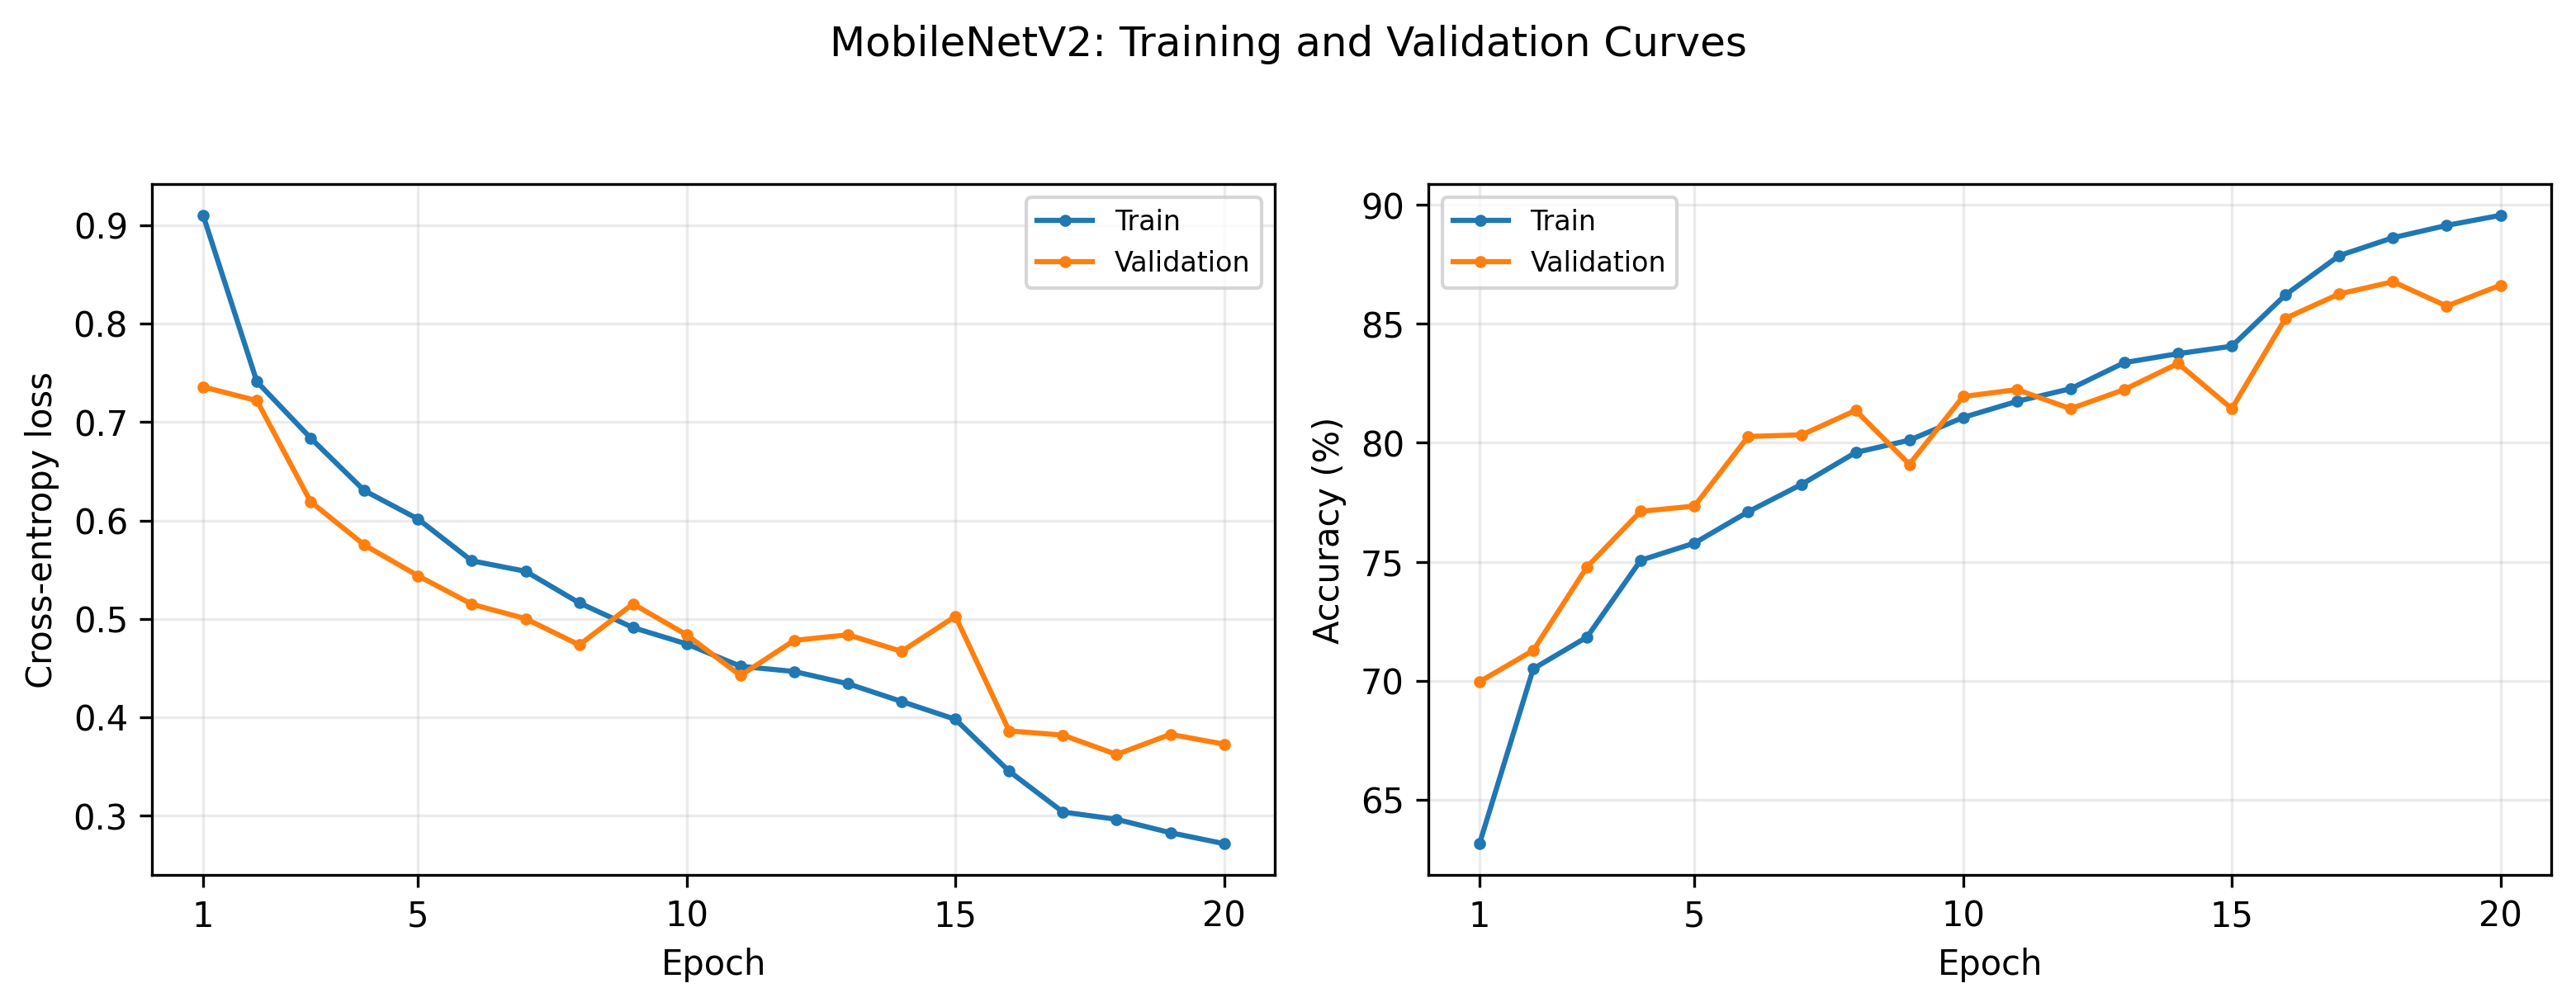
\includegraphics[width=\linewidth]{task5/mobilenet_v2_training_curves.png}
\caption{MobileNetV2.}
\end{subfigure}\hfill
\begin{subfigure}{0.49\linewidth}\centering
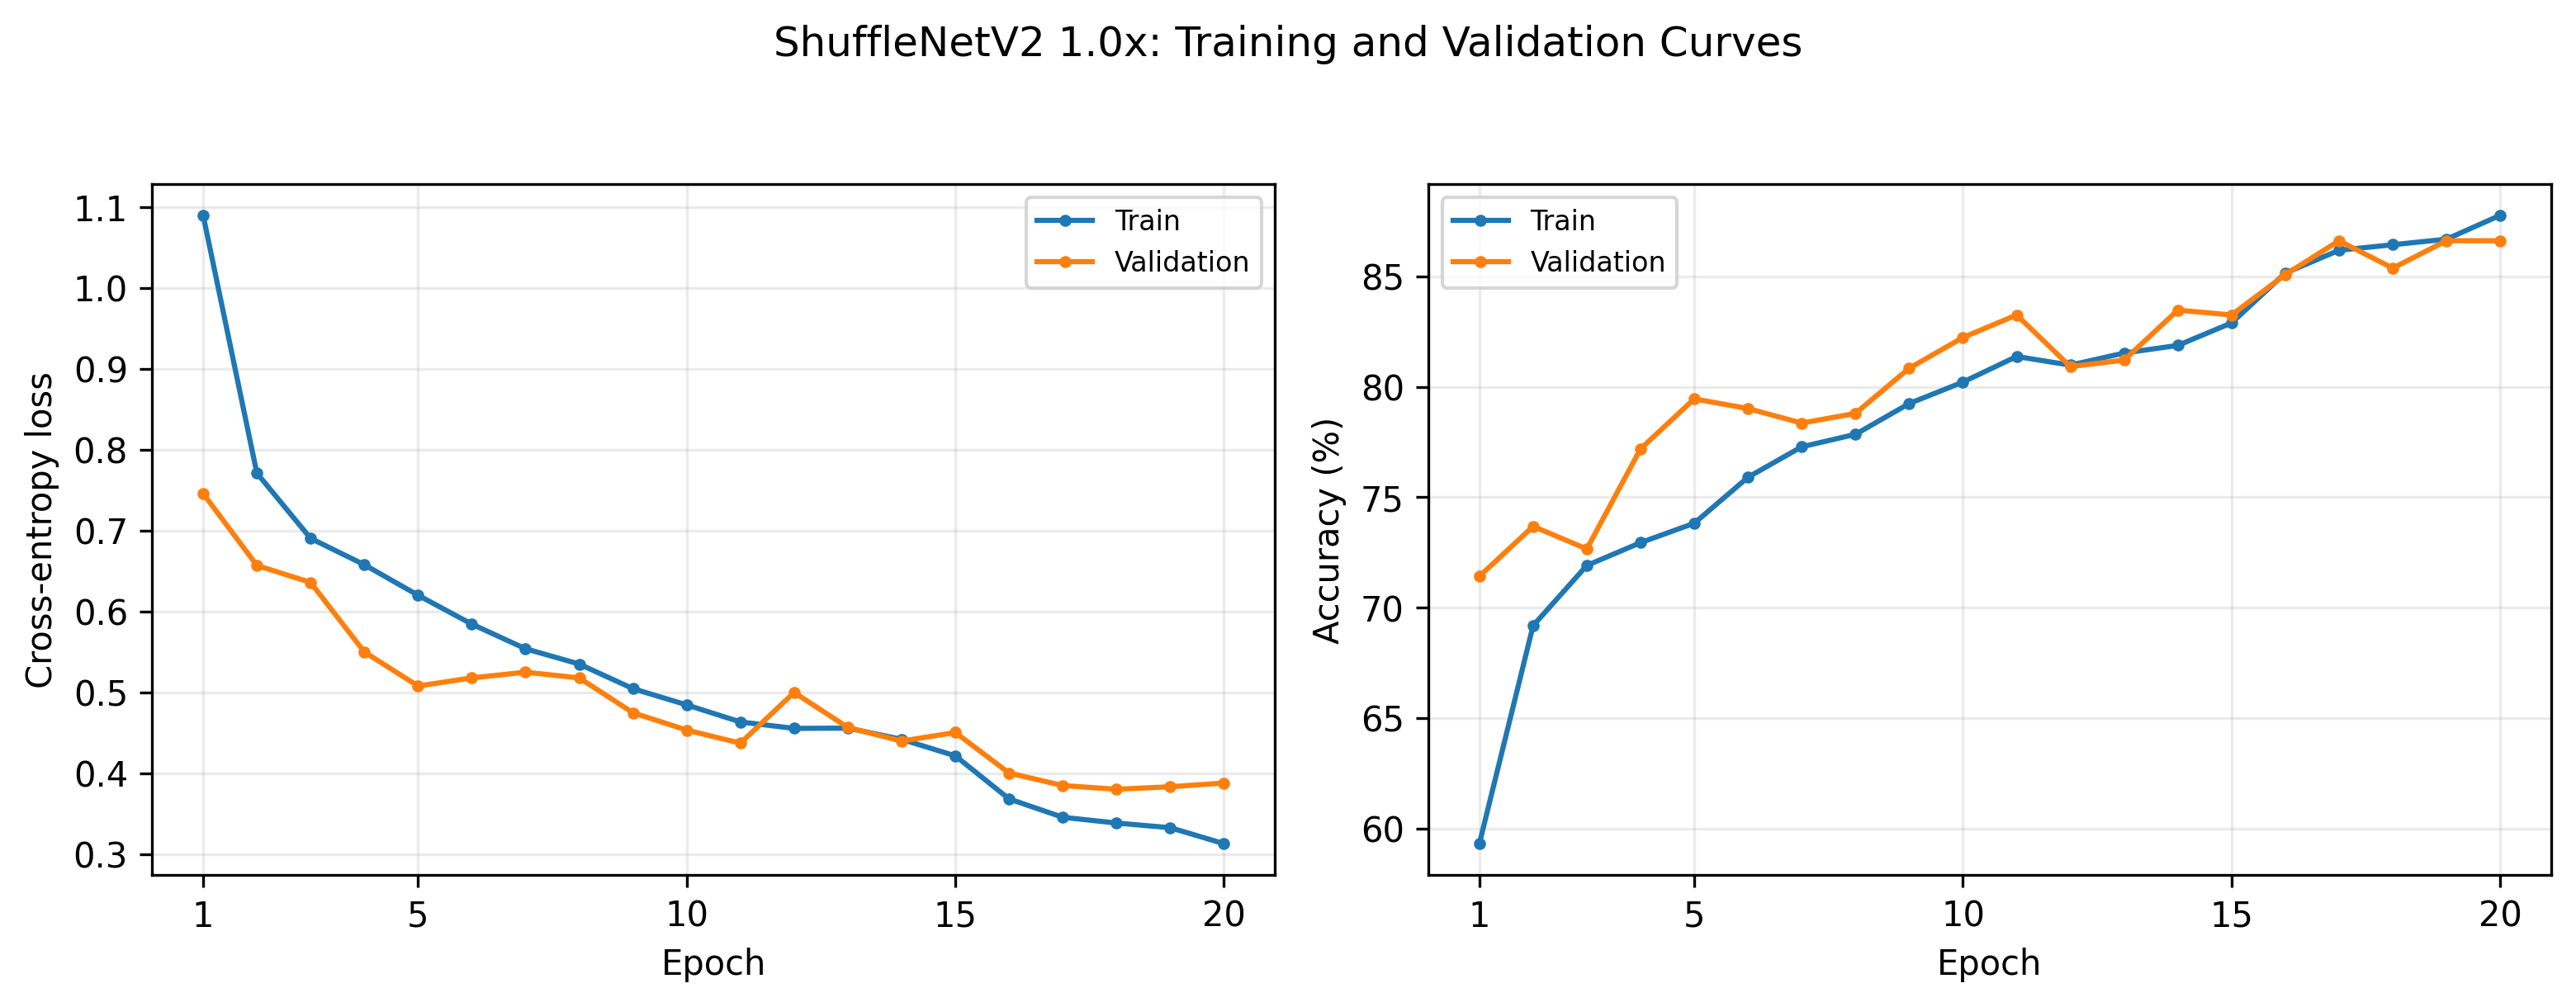
\includegraphics[width=\linewidth]{task5/shufflenet_v2_training_curves.png}
\caption{ShuffleNetV2 1.0x.}
\end{subfigure}
\caption{Fine-tuning and validation curves for the two pre-trained models.}
\end{figure}

\begin{figure}[H]
\centering
\begin{subfigure}{0.49\linewidth}\centering
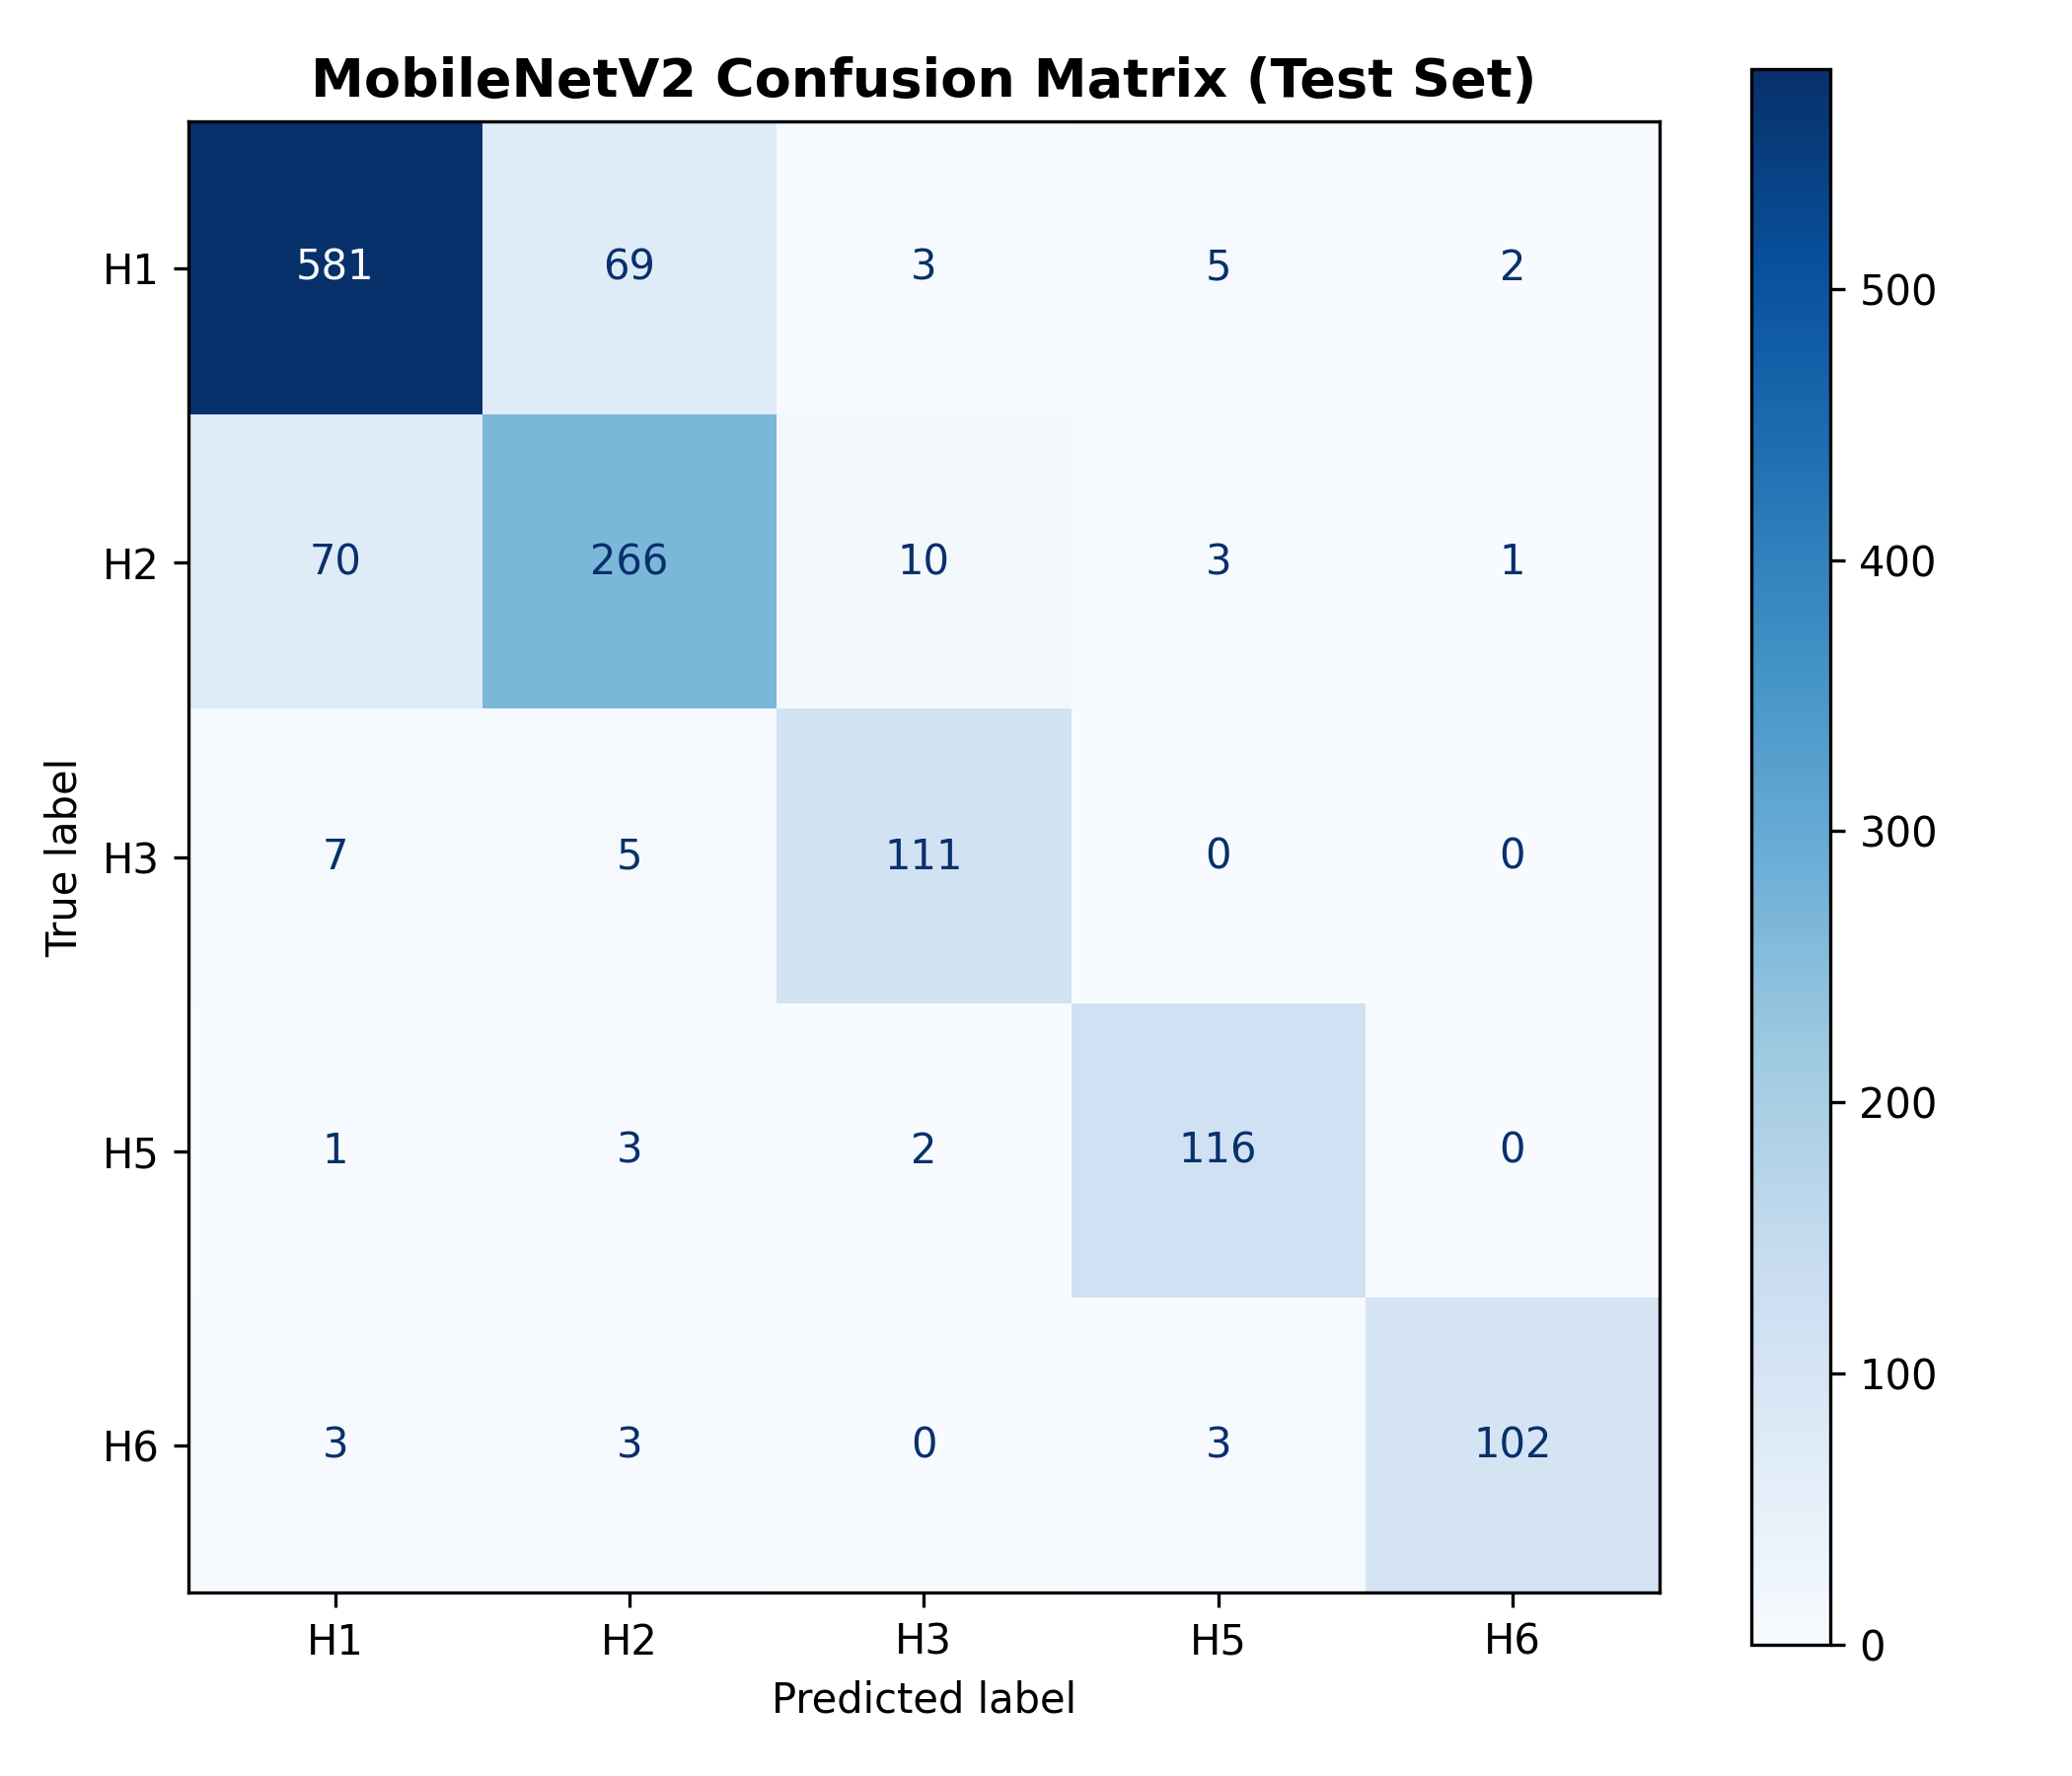
\includegraphics[width=\linewidth]{task5/mobilenet_v2_confusion_matrix.png}
\caption{MobileNetV2.}
\end{subfigure}\hfill
\begin{subfigure}{0.49\linewidth}\centering
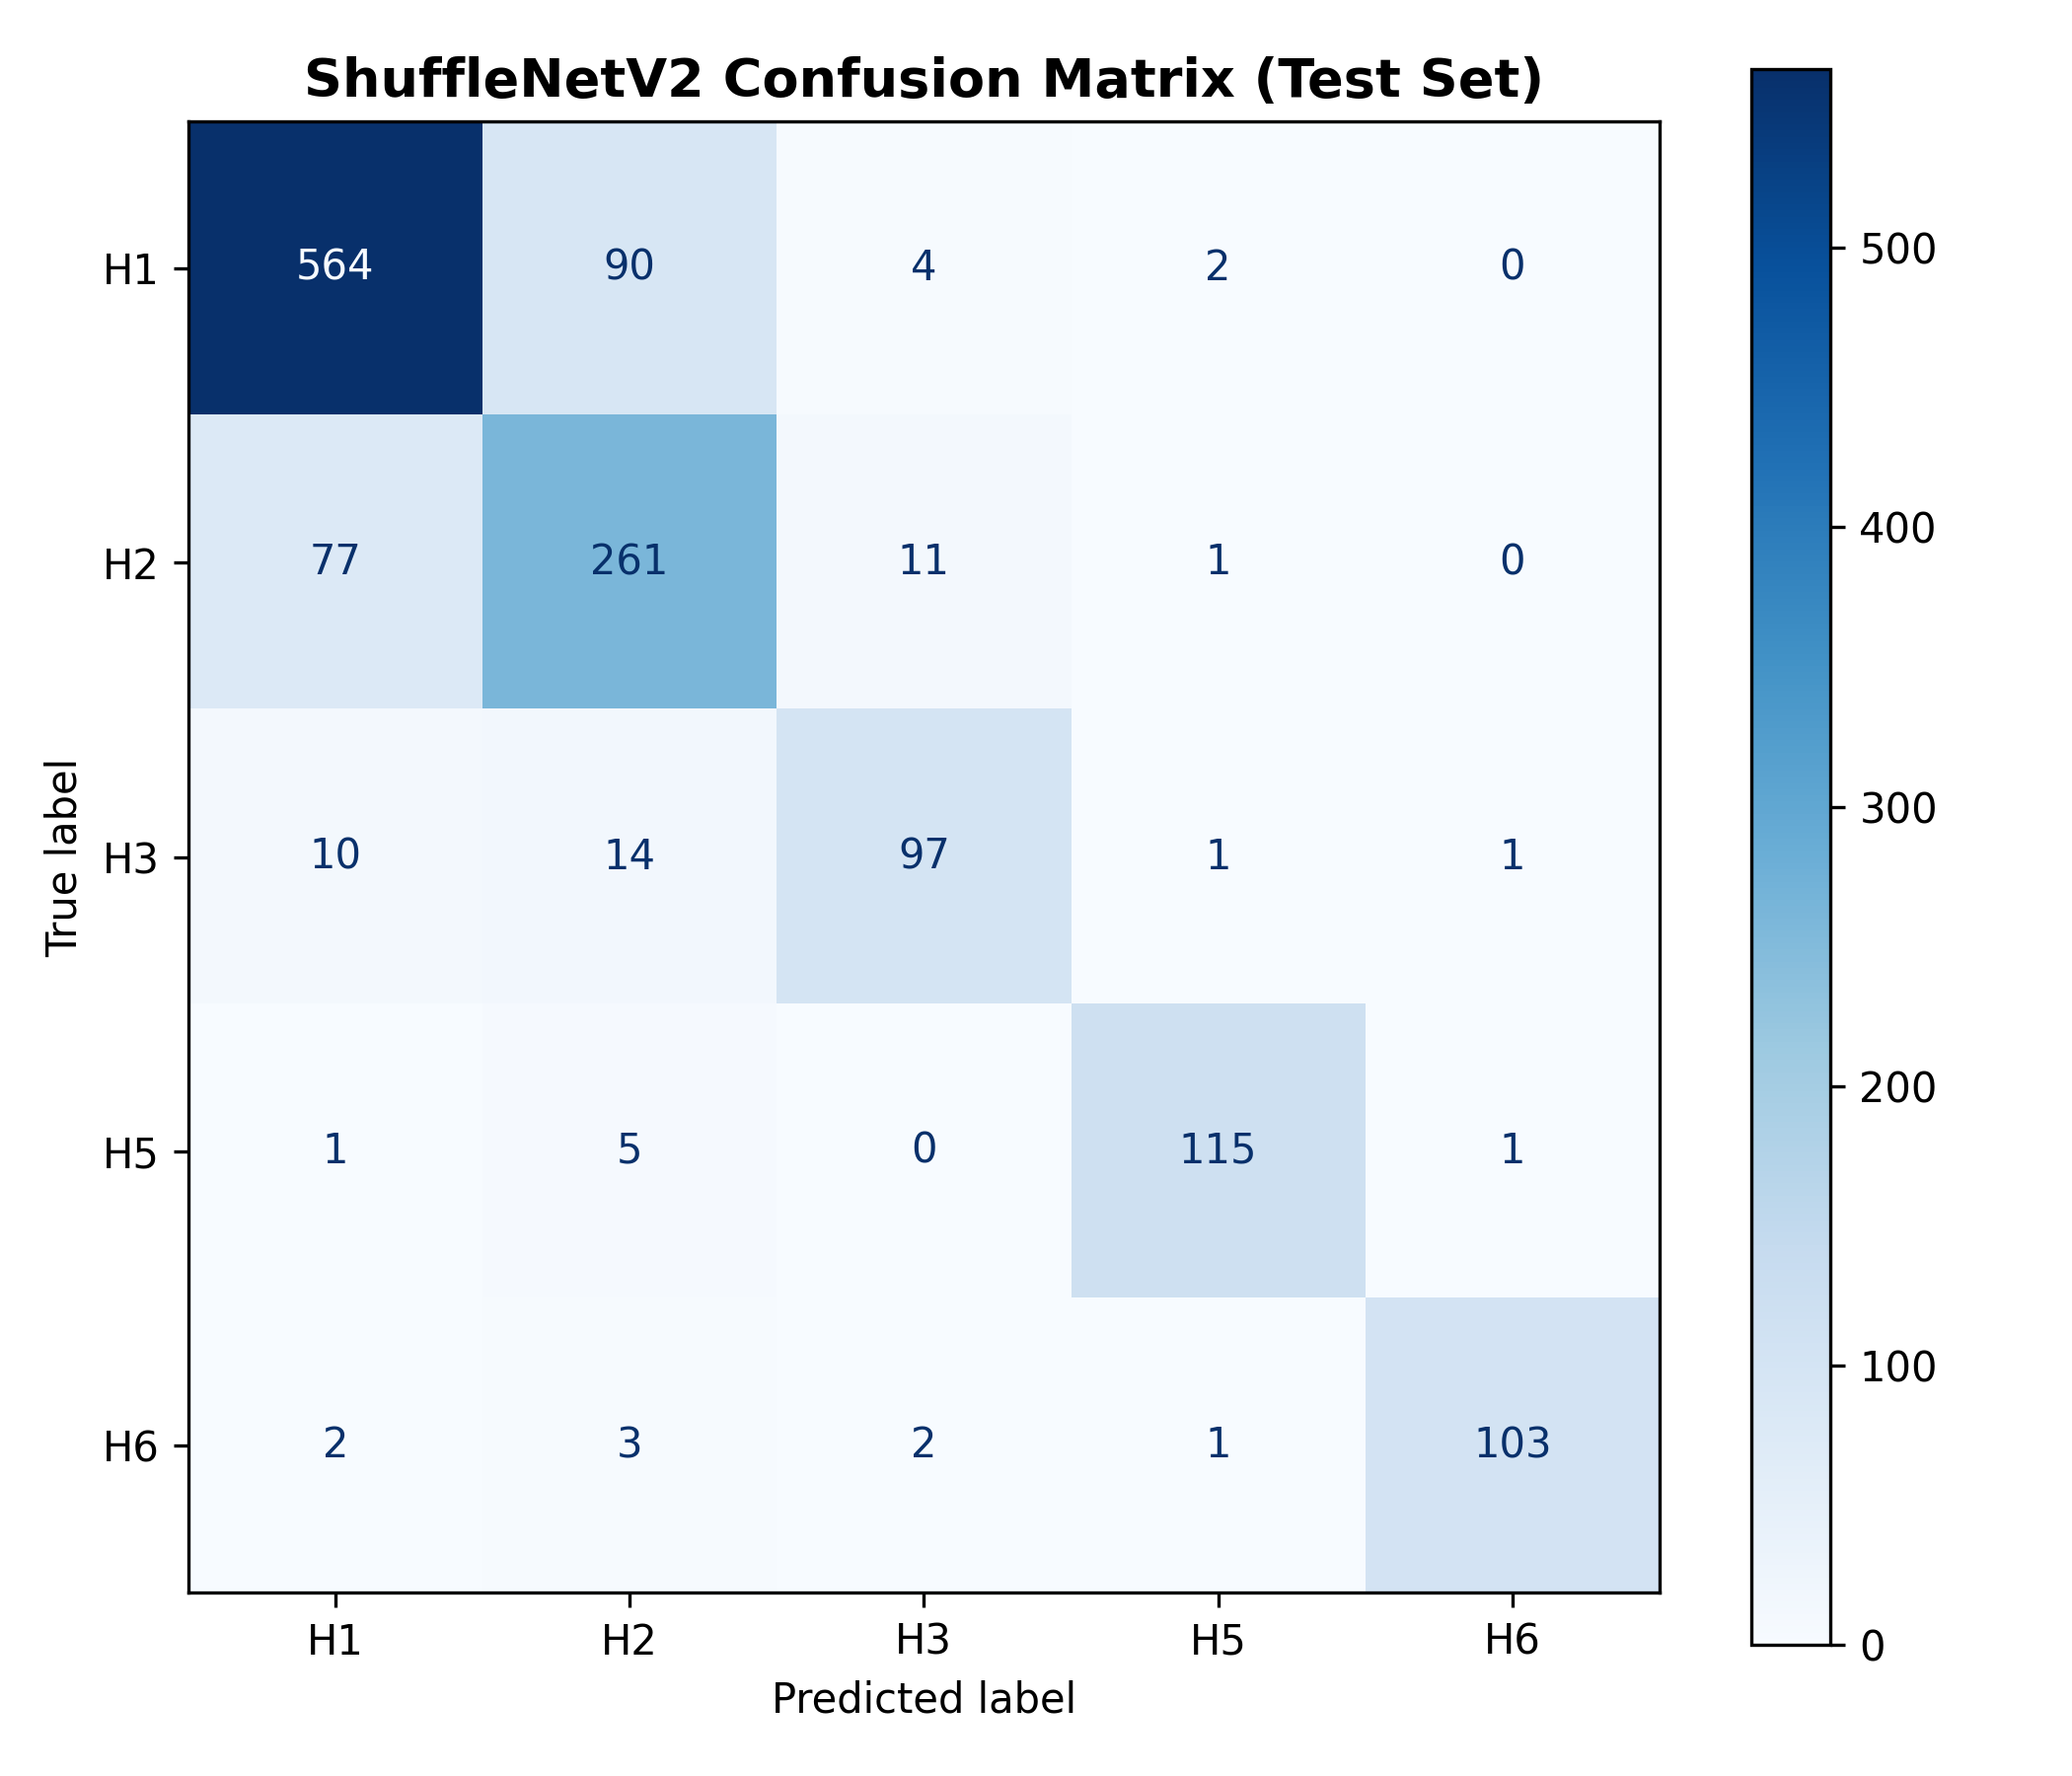
\includegraphics[width=\linewidth]{task5/shufflenet_v2_confusion_matrix.png}
\caption{ShuffleNetV2 1.0x.}
\end{subfigure}
\caption{Corrected test-set confusion matrices for the fine-tuned models.}
\end{figure}

\begin{table}[H]
\centering
\scriptsize
\caption{Canonical clean-split Task 5 results.}
\resizebox{\textwidth}{!}{%
\begin{tabular}{lrrrrrrrrrrr}
\toprule
Model & Params & Size & Loss & Accuracy & Macro P & Macro R & Macro F1 & Total time & Time/ep & MACs/FLOPs\\
\midrule
MobileNetV2 & \MobileParams & \MobileSizeMiB\ MiB & \MobileTestLoss & \MobileAccuracy\% & \MobilePrecision & \MobileRecall & \MobileFOne & \MobileTotalTime\ s & \MobileEpochTime\ s & \MobileMACs/\MobileFLOPs\ M\\
ShuffleNetV2 1.0x & \ShuffleParams & \ShuffleSizeMiB\ MiB & \ShuffleTestLoss & \ShuffleAccuracy\% & \ShufflePrecision & \ShuffleRecall & \ShuffleFOne & \ShuffleTotalTime\ s & \ShuffleEpochTime\ s & \ShuffleMACs/\ShuffleFLOPs\ M\\
\bottomrule
\end{tabular}}
\end{table}

MobileNetV2 gives the highest accuracy and macro F1. ShuffleNetV2 is smaller and uses fewer MACs while still substantially outperforming Model B. Pre-training likely contributes reusable visual representations, but the advantage cannot be assigned to pre-training alone because architecture and capacity also differ.

\section{Task 6: Final Comparison and Trade-off Discussion}
\subsection{Accuracy, storage, and computation}
\begin{figure}[H]
\centering
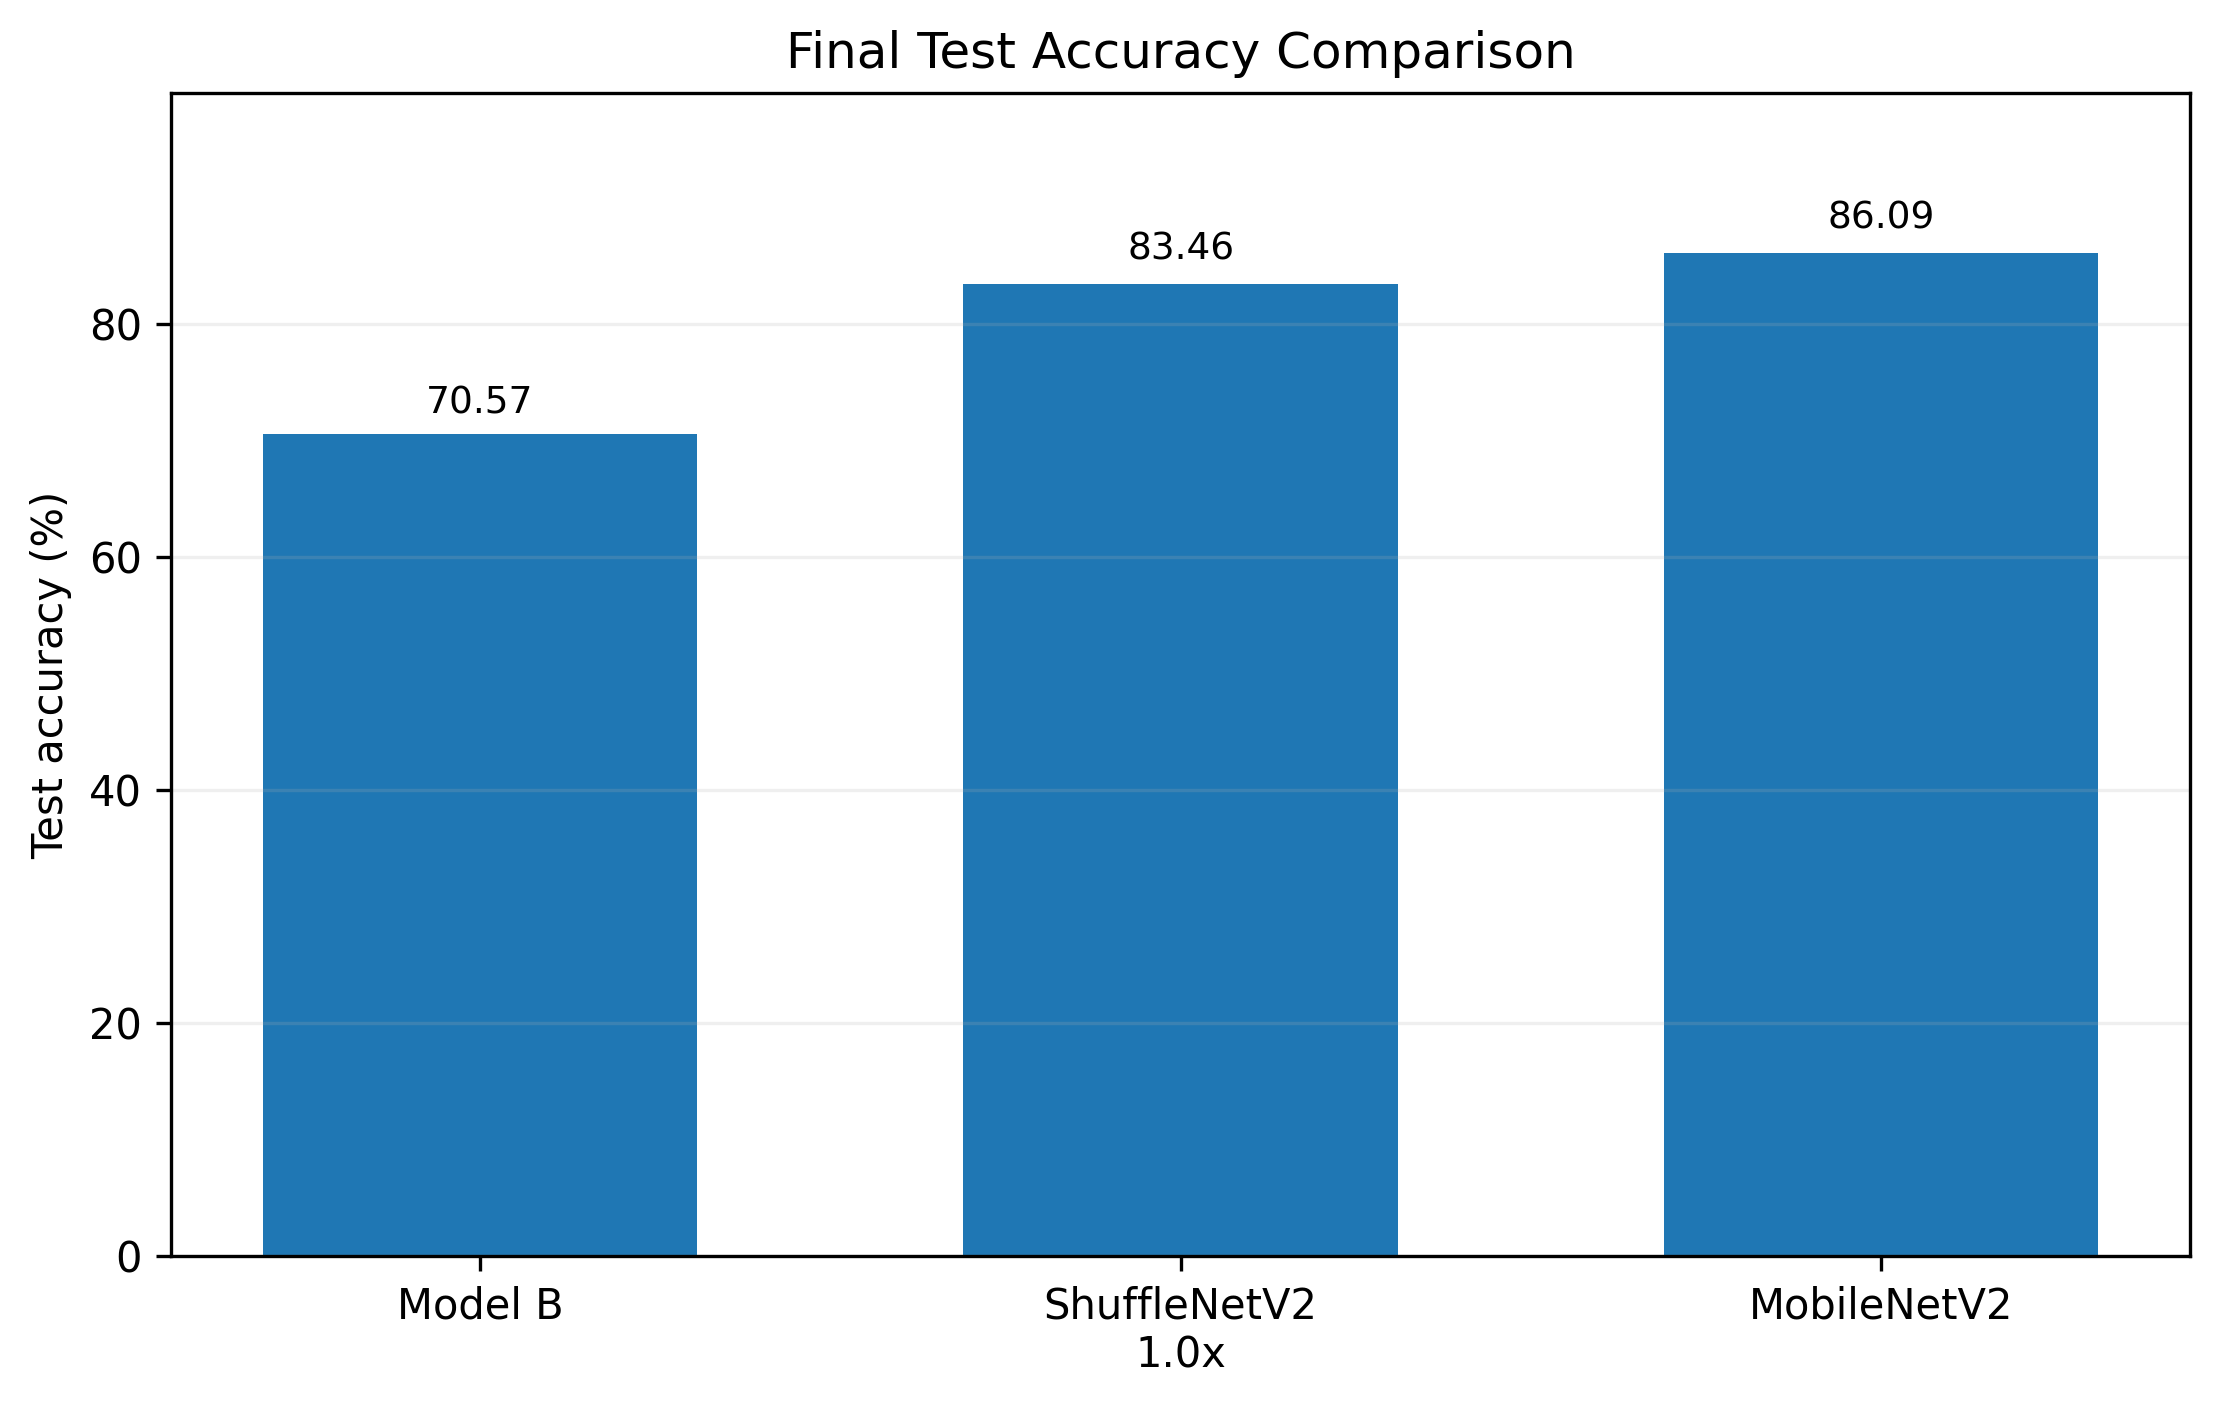
\includegraphics[width=0.72\linewidth]{task6/test_accuracy_comparison.png}
\caption{Corrected test accuracy for Model B and the two fine-tuned pre-trained models.}
\end{figure}

MobileNetV2 improves on Model B by \MobileAccuracyGainVsB{} percentage points; ShuffleNetV2 improves by \ShuffleAccuracyGainVsB{} points. Their H2 recalls are \MobileHTwoRecall{} and \ShuffleHTwoRecall, compared with \ModelBHTwoRecall{} for Model B.

\begin{figure}[H]
\centering
\begin{subfigure}{0.49\linewidth}\centering
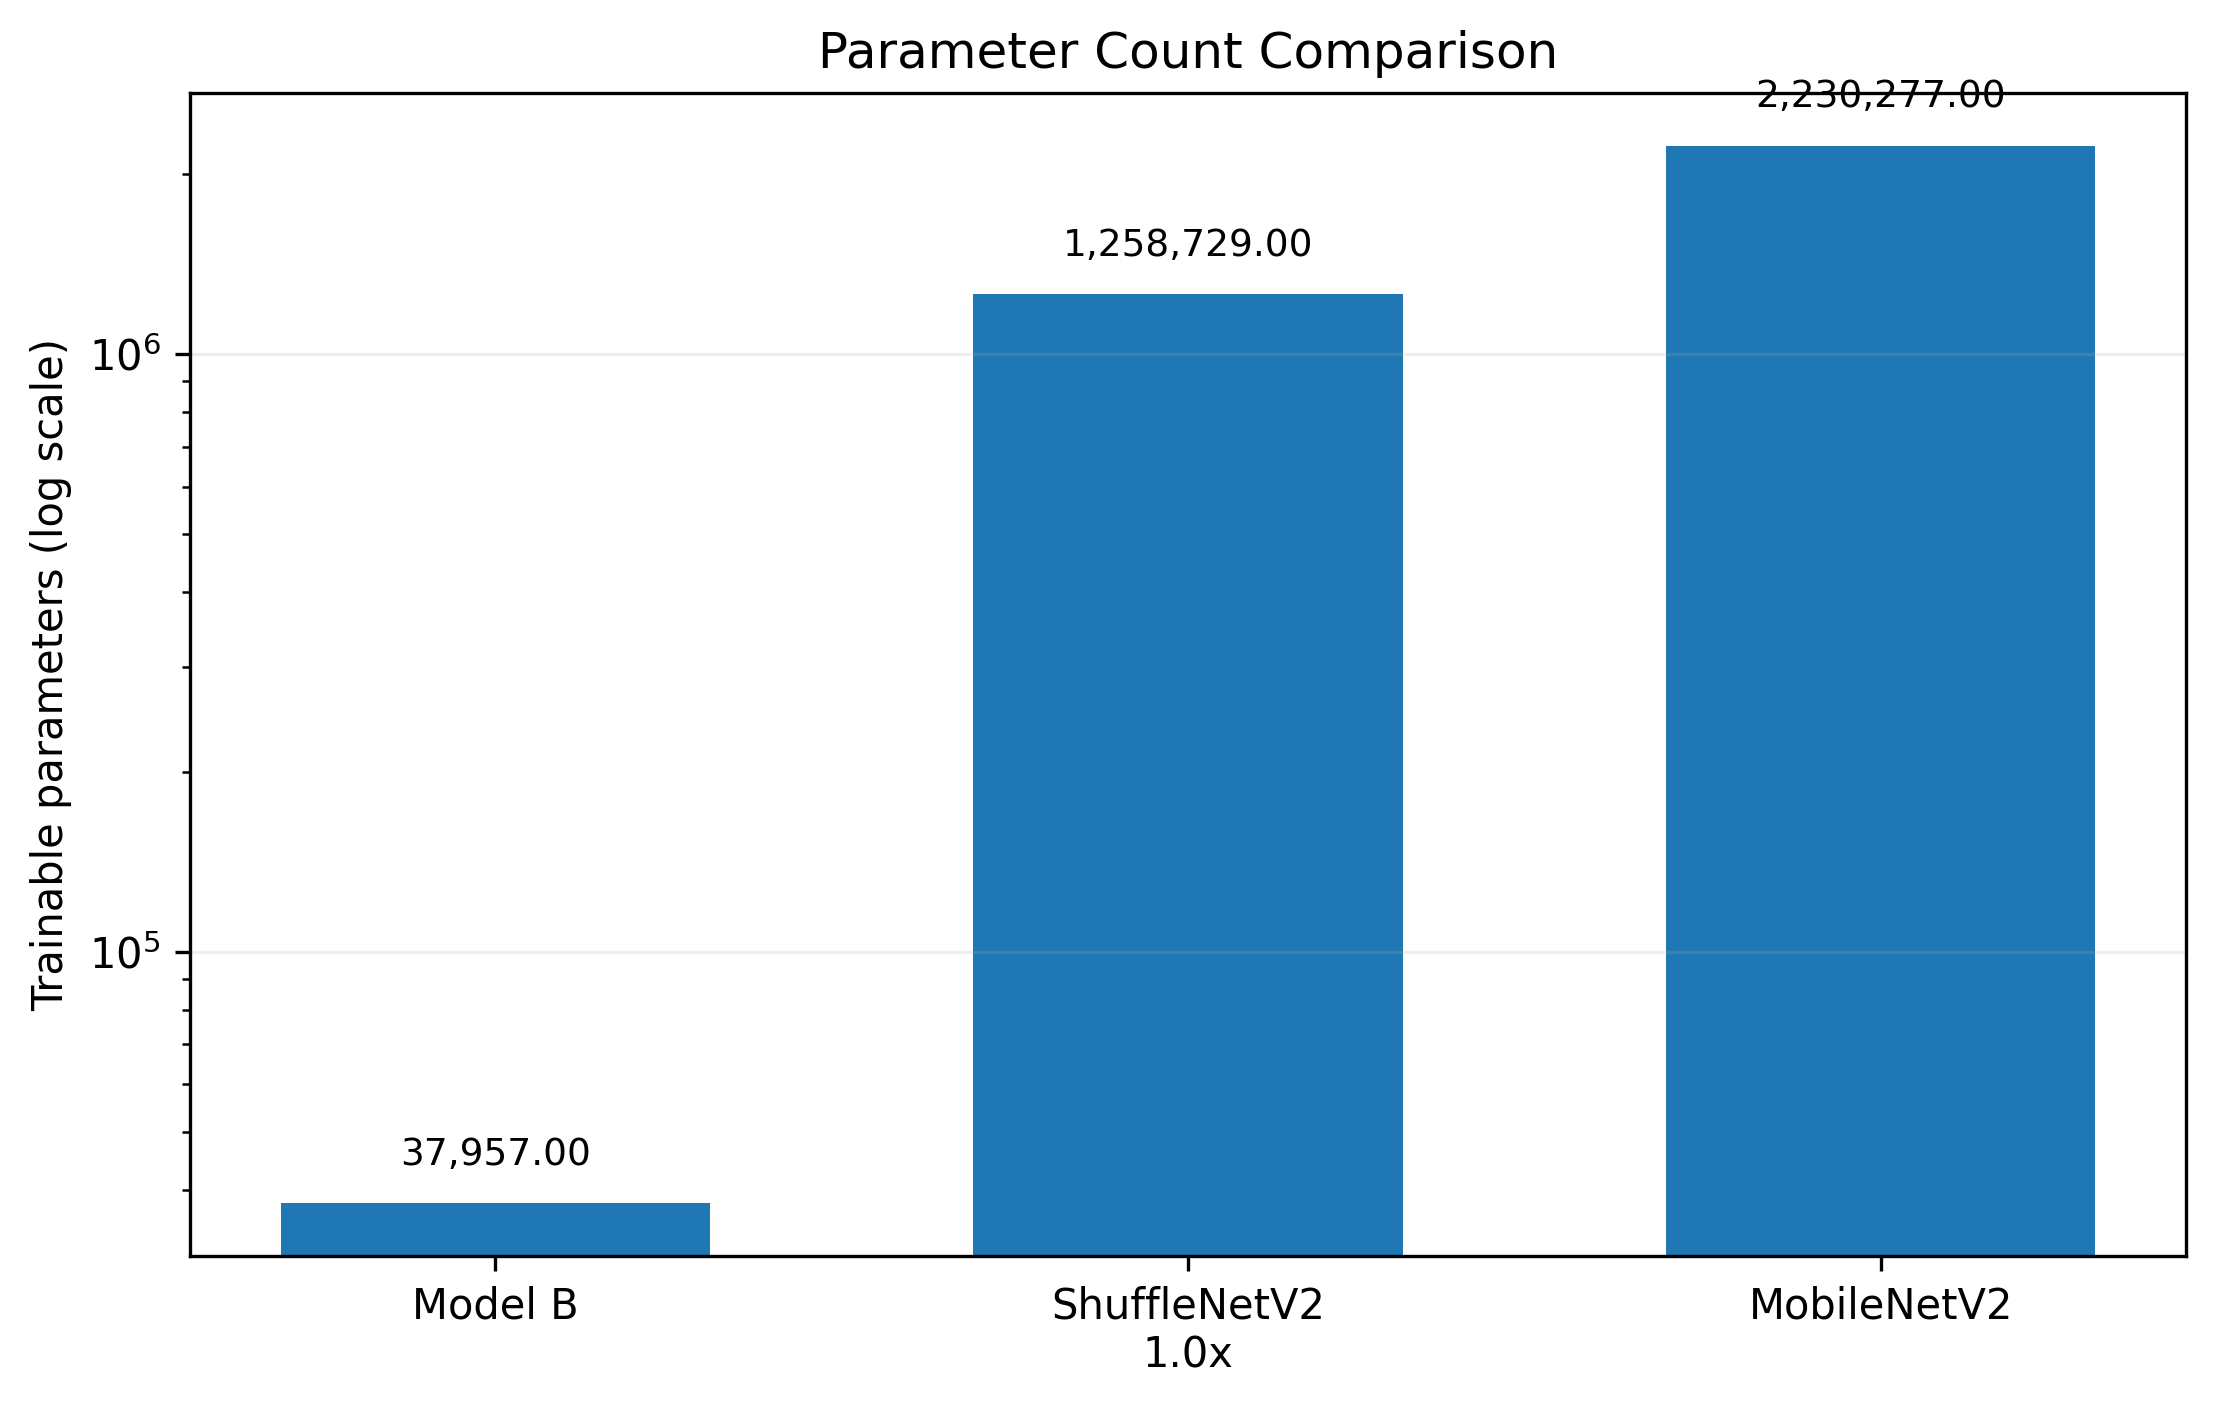
\includegraphics[width=\linewidth]{task6/parameter_count_comparison.png}
\caption{Trainable parameters.}
\end{subfigure}\hfill
\begin{subfigure}{0.49\linewidth}\centering
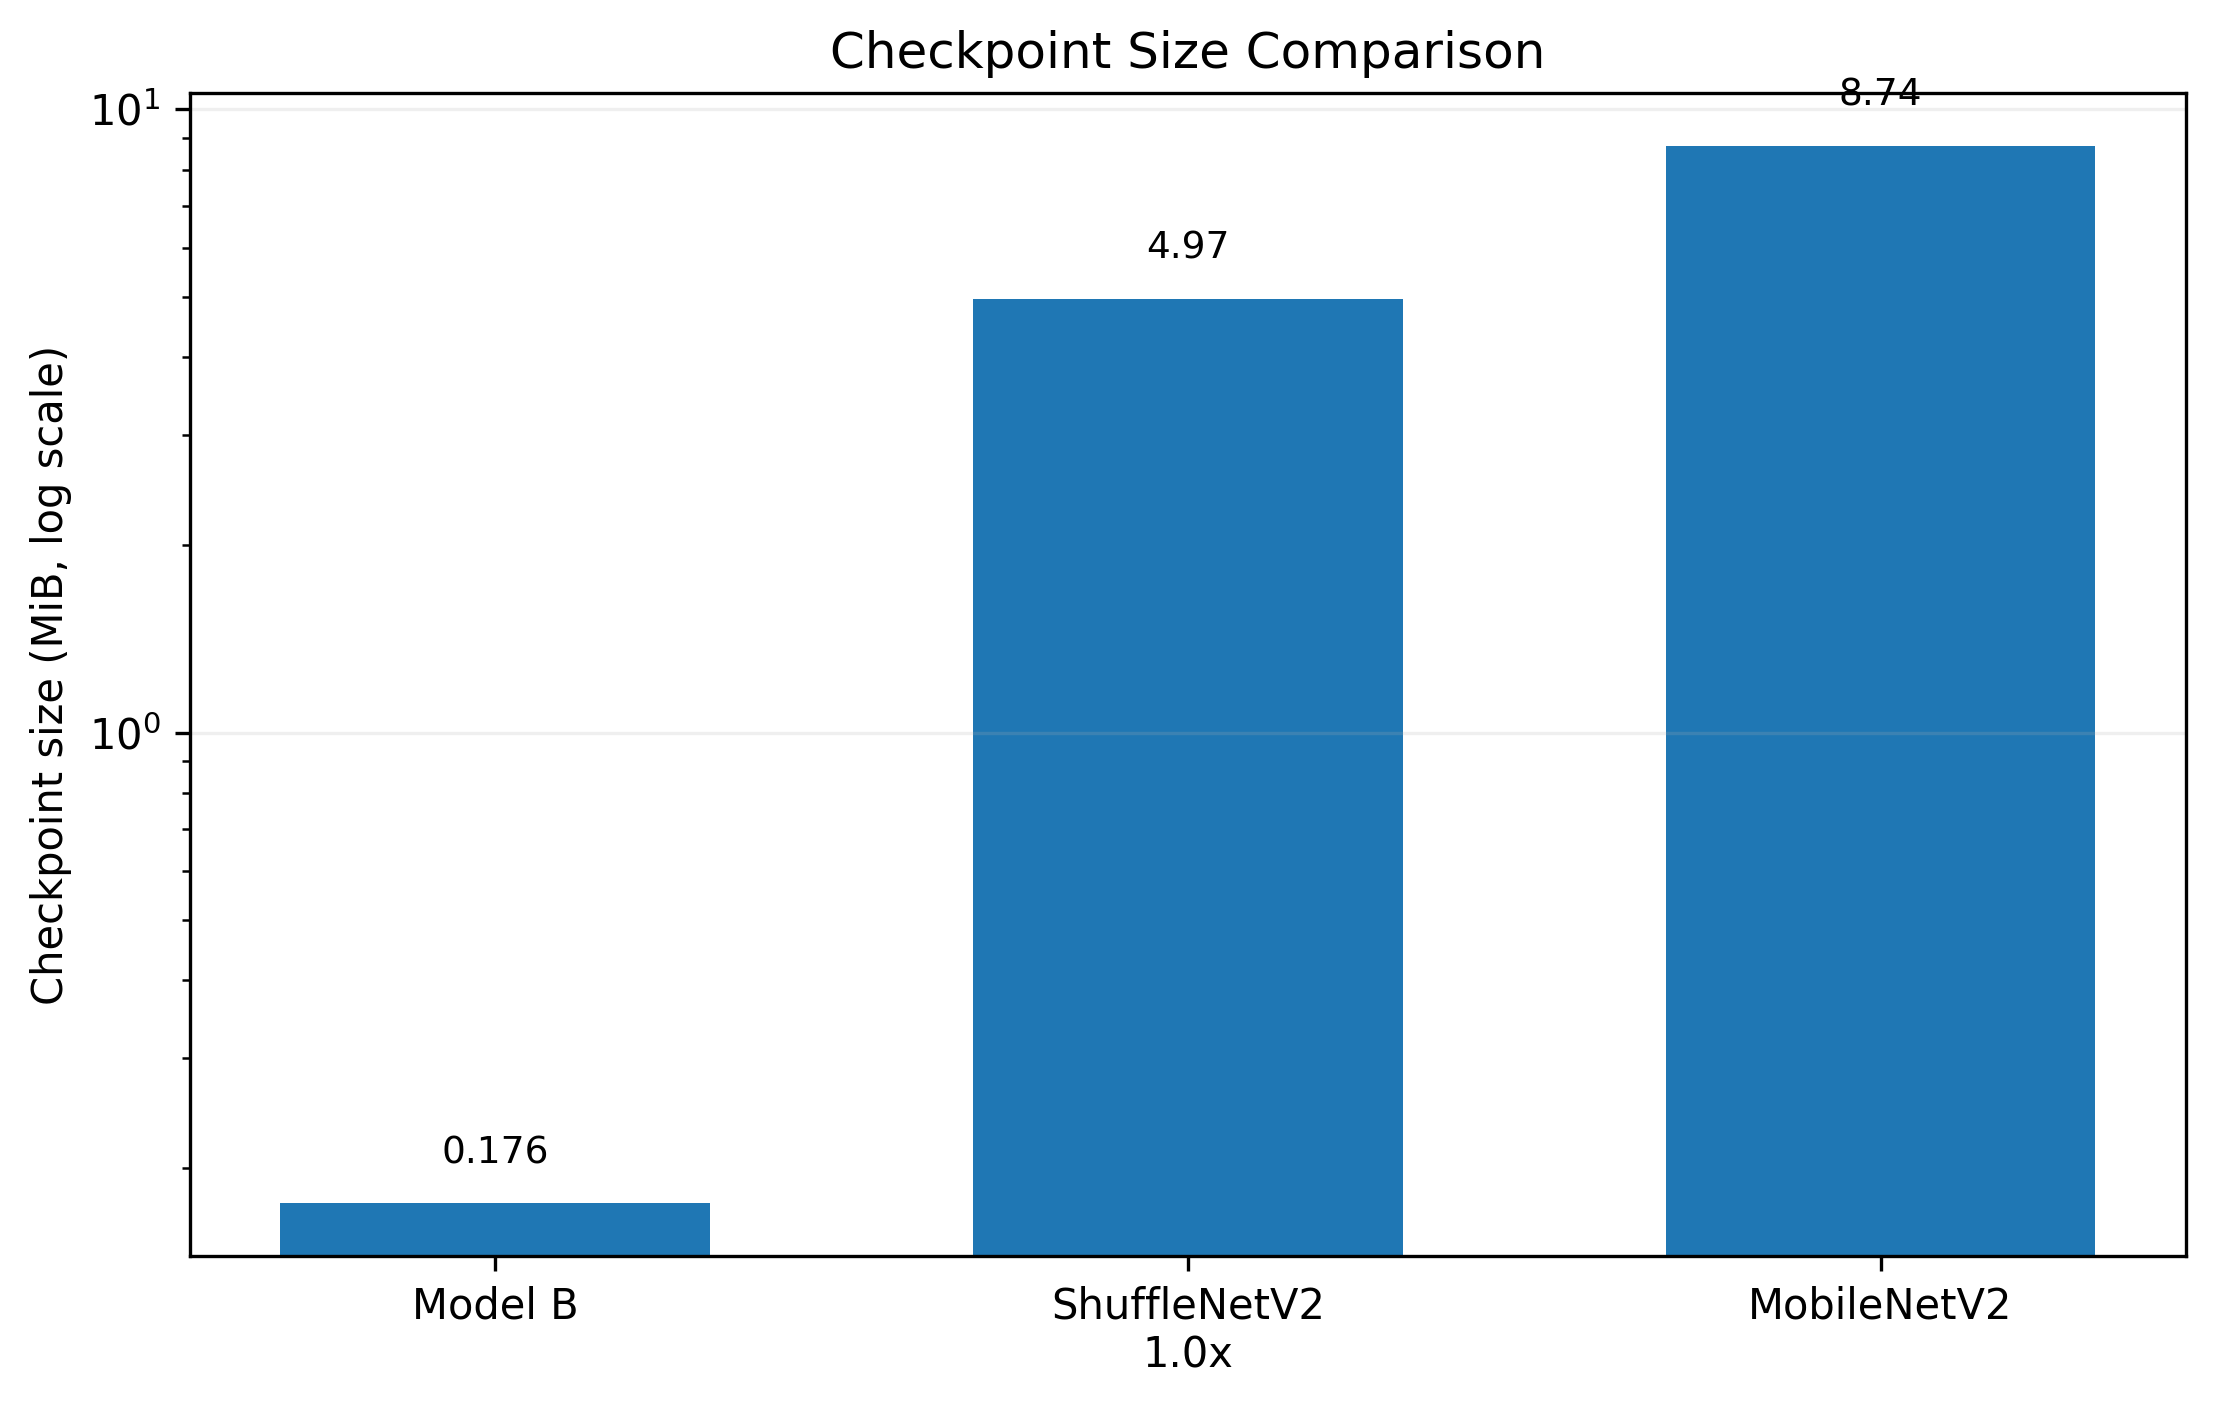
\includegraphics[width=\linewidth]{task6/model_size_comparison.png}
\caption{Checkpoint storage in MiB.}
\end{subfigure}
\caption{Parameter and actual checkpoint-size comparisons. Log scales expose the large ratios.}
\end{figure}

Relative to Model B, MobileNetV2 has \MobileParamFactorVsB$\times$ the parameters and a \MobileSizeFactorVsB$\times$ larger checkpoint. ShuffleNetV2 has \ShuffleParamFactorVsB$\times$ the parameters and a \ShuffleSizeFactorVsB$\times$ larger checkpoint.

\begin{figure}[H]
\centering
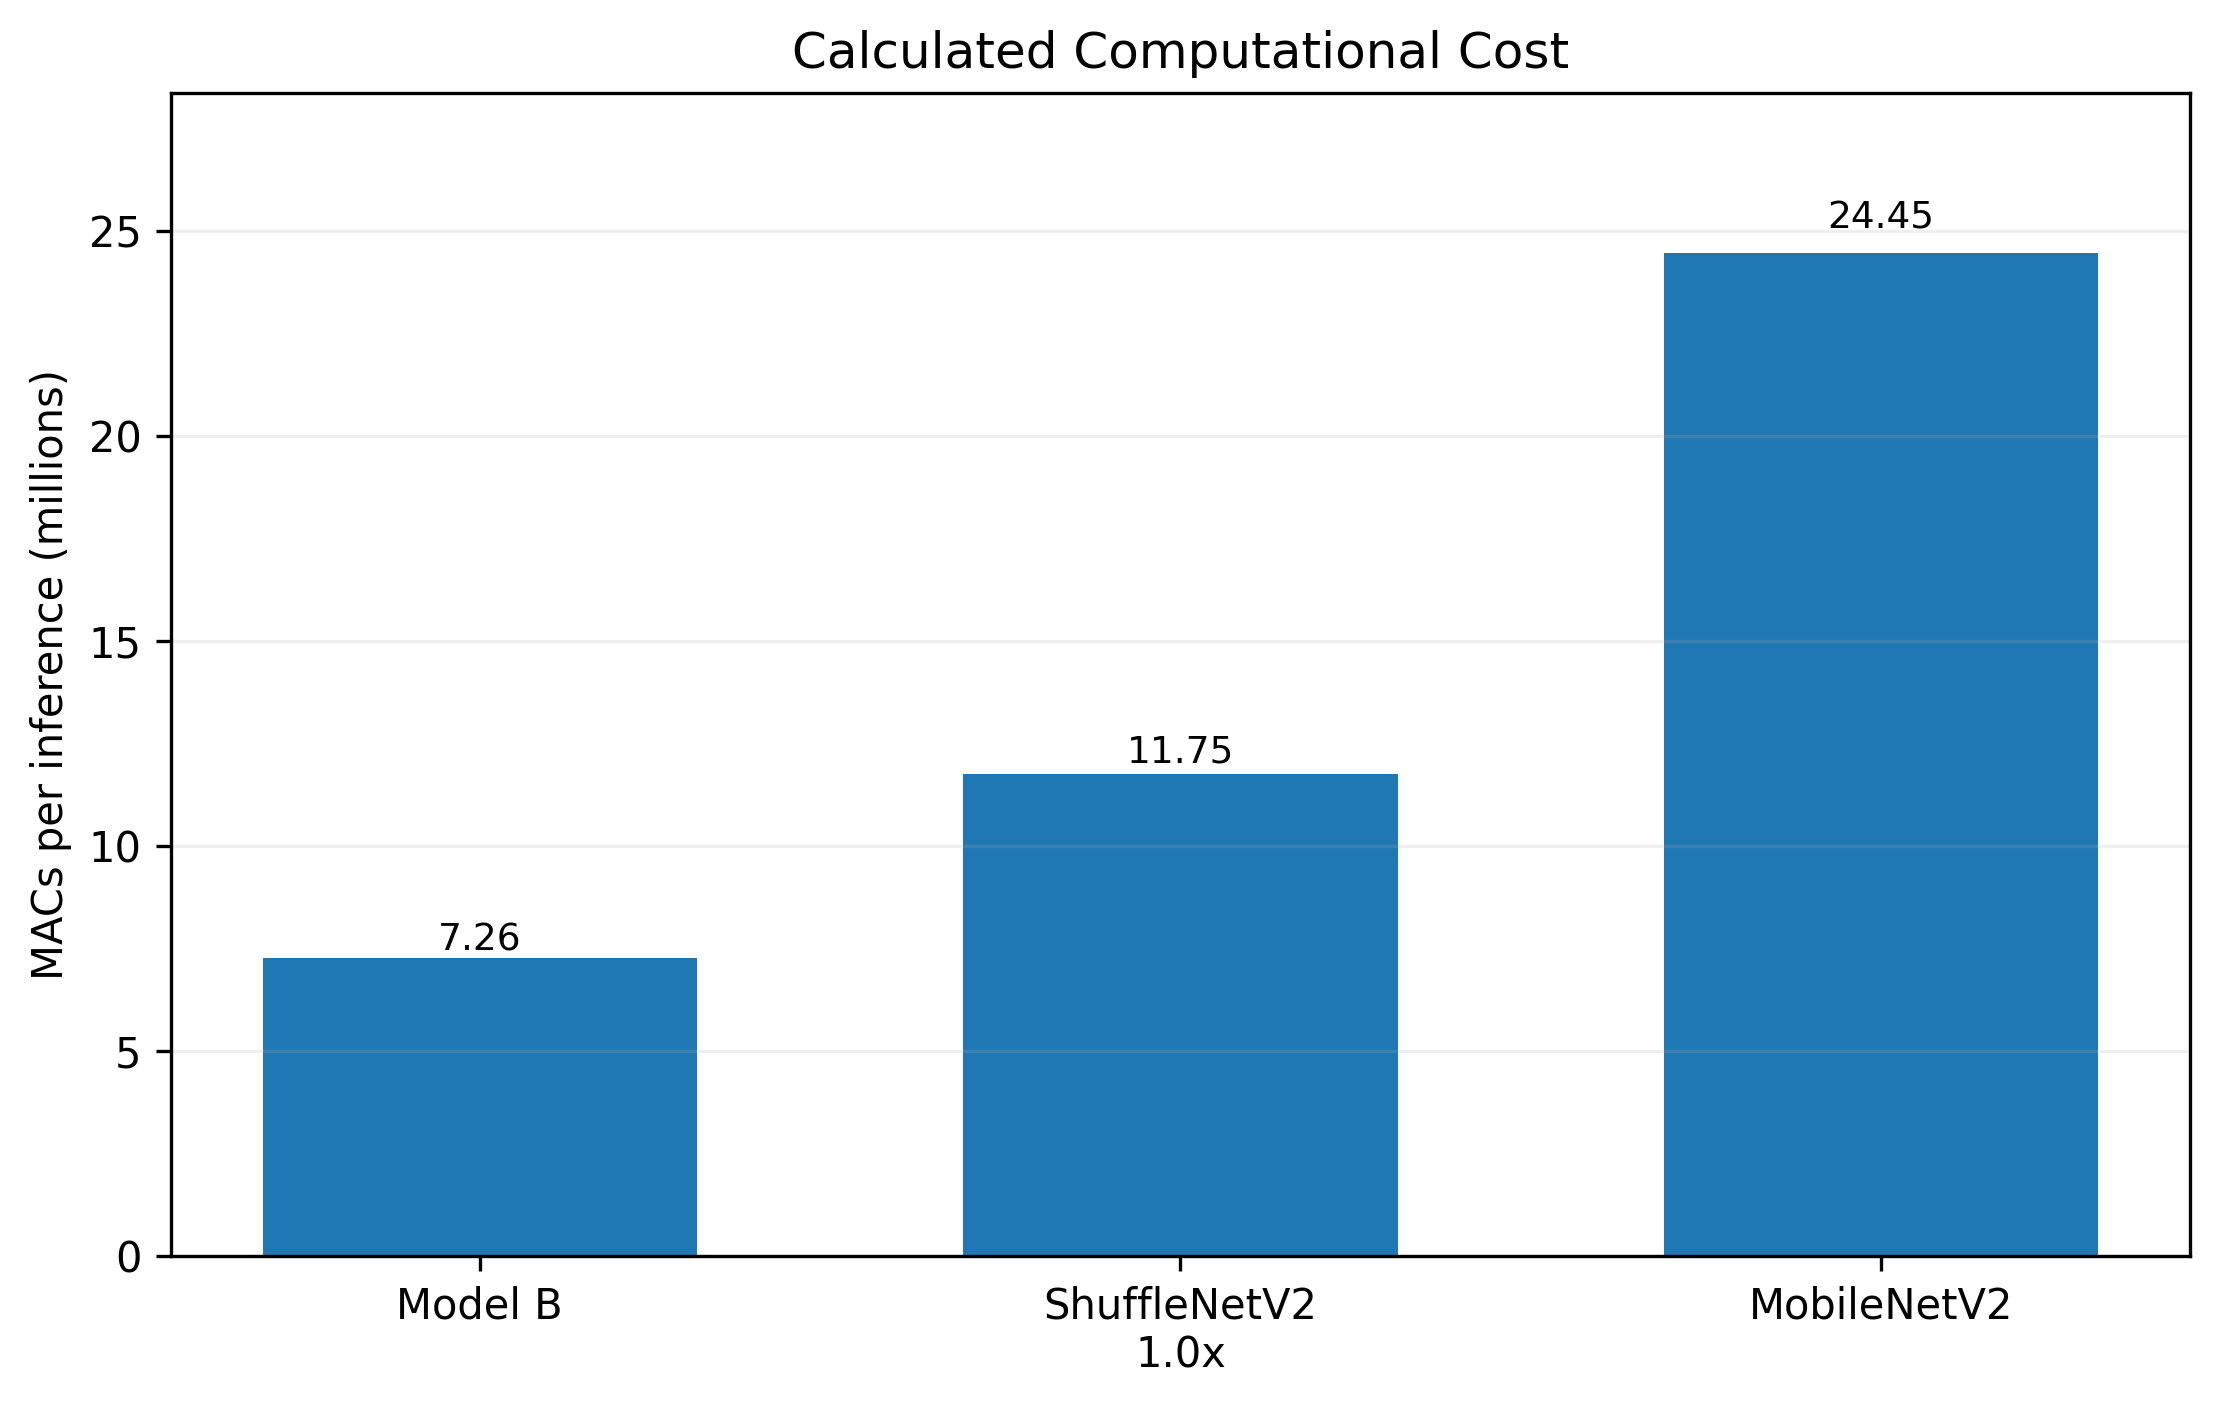
\includegraphics[width=0.72\linewidth]{task6/mac_comparison.png}
\caption{Calculated Conv2d/Linear MACs per $64\times64$ image.}
\end{figure}

MobileNetV2 uses \MobileMACFactorVsB$\times$ Model B's MAC count and ShuffleNetV2 uses \ShuffleMACFactorVsB$\times$. Model B is therefore the lowest-cost custom option, whereas the pre-trained models combine larger capacity, different efficient building blocks, and learned ImageNet representations to obtain higher accuracy.

\subsection{Accuracy-efficiency frontier}
\begin{figure}[H]
\centering
\begin{subfigure}{0.49\linewidth}\centering
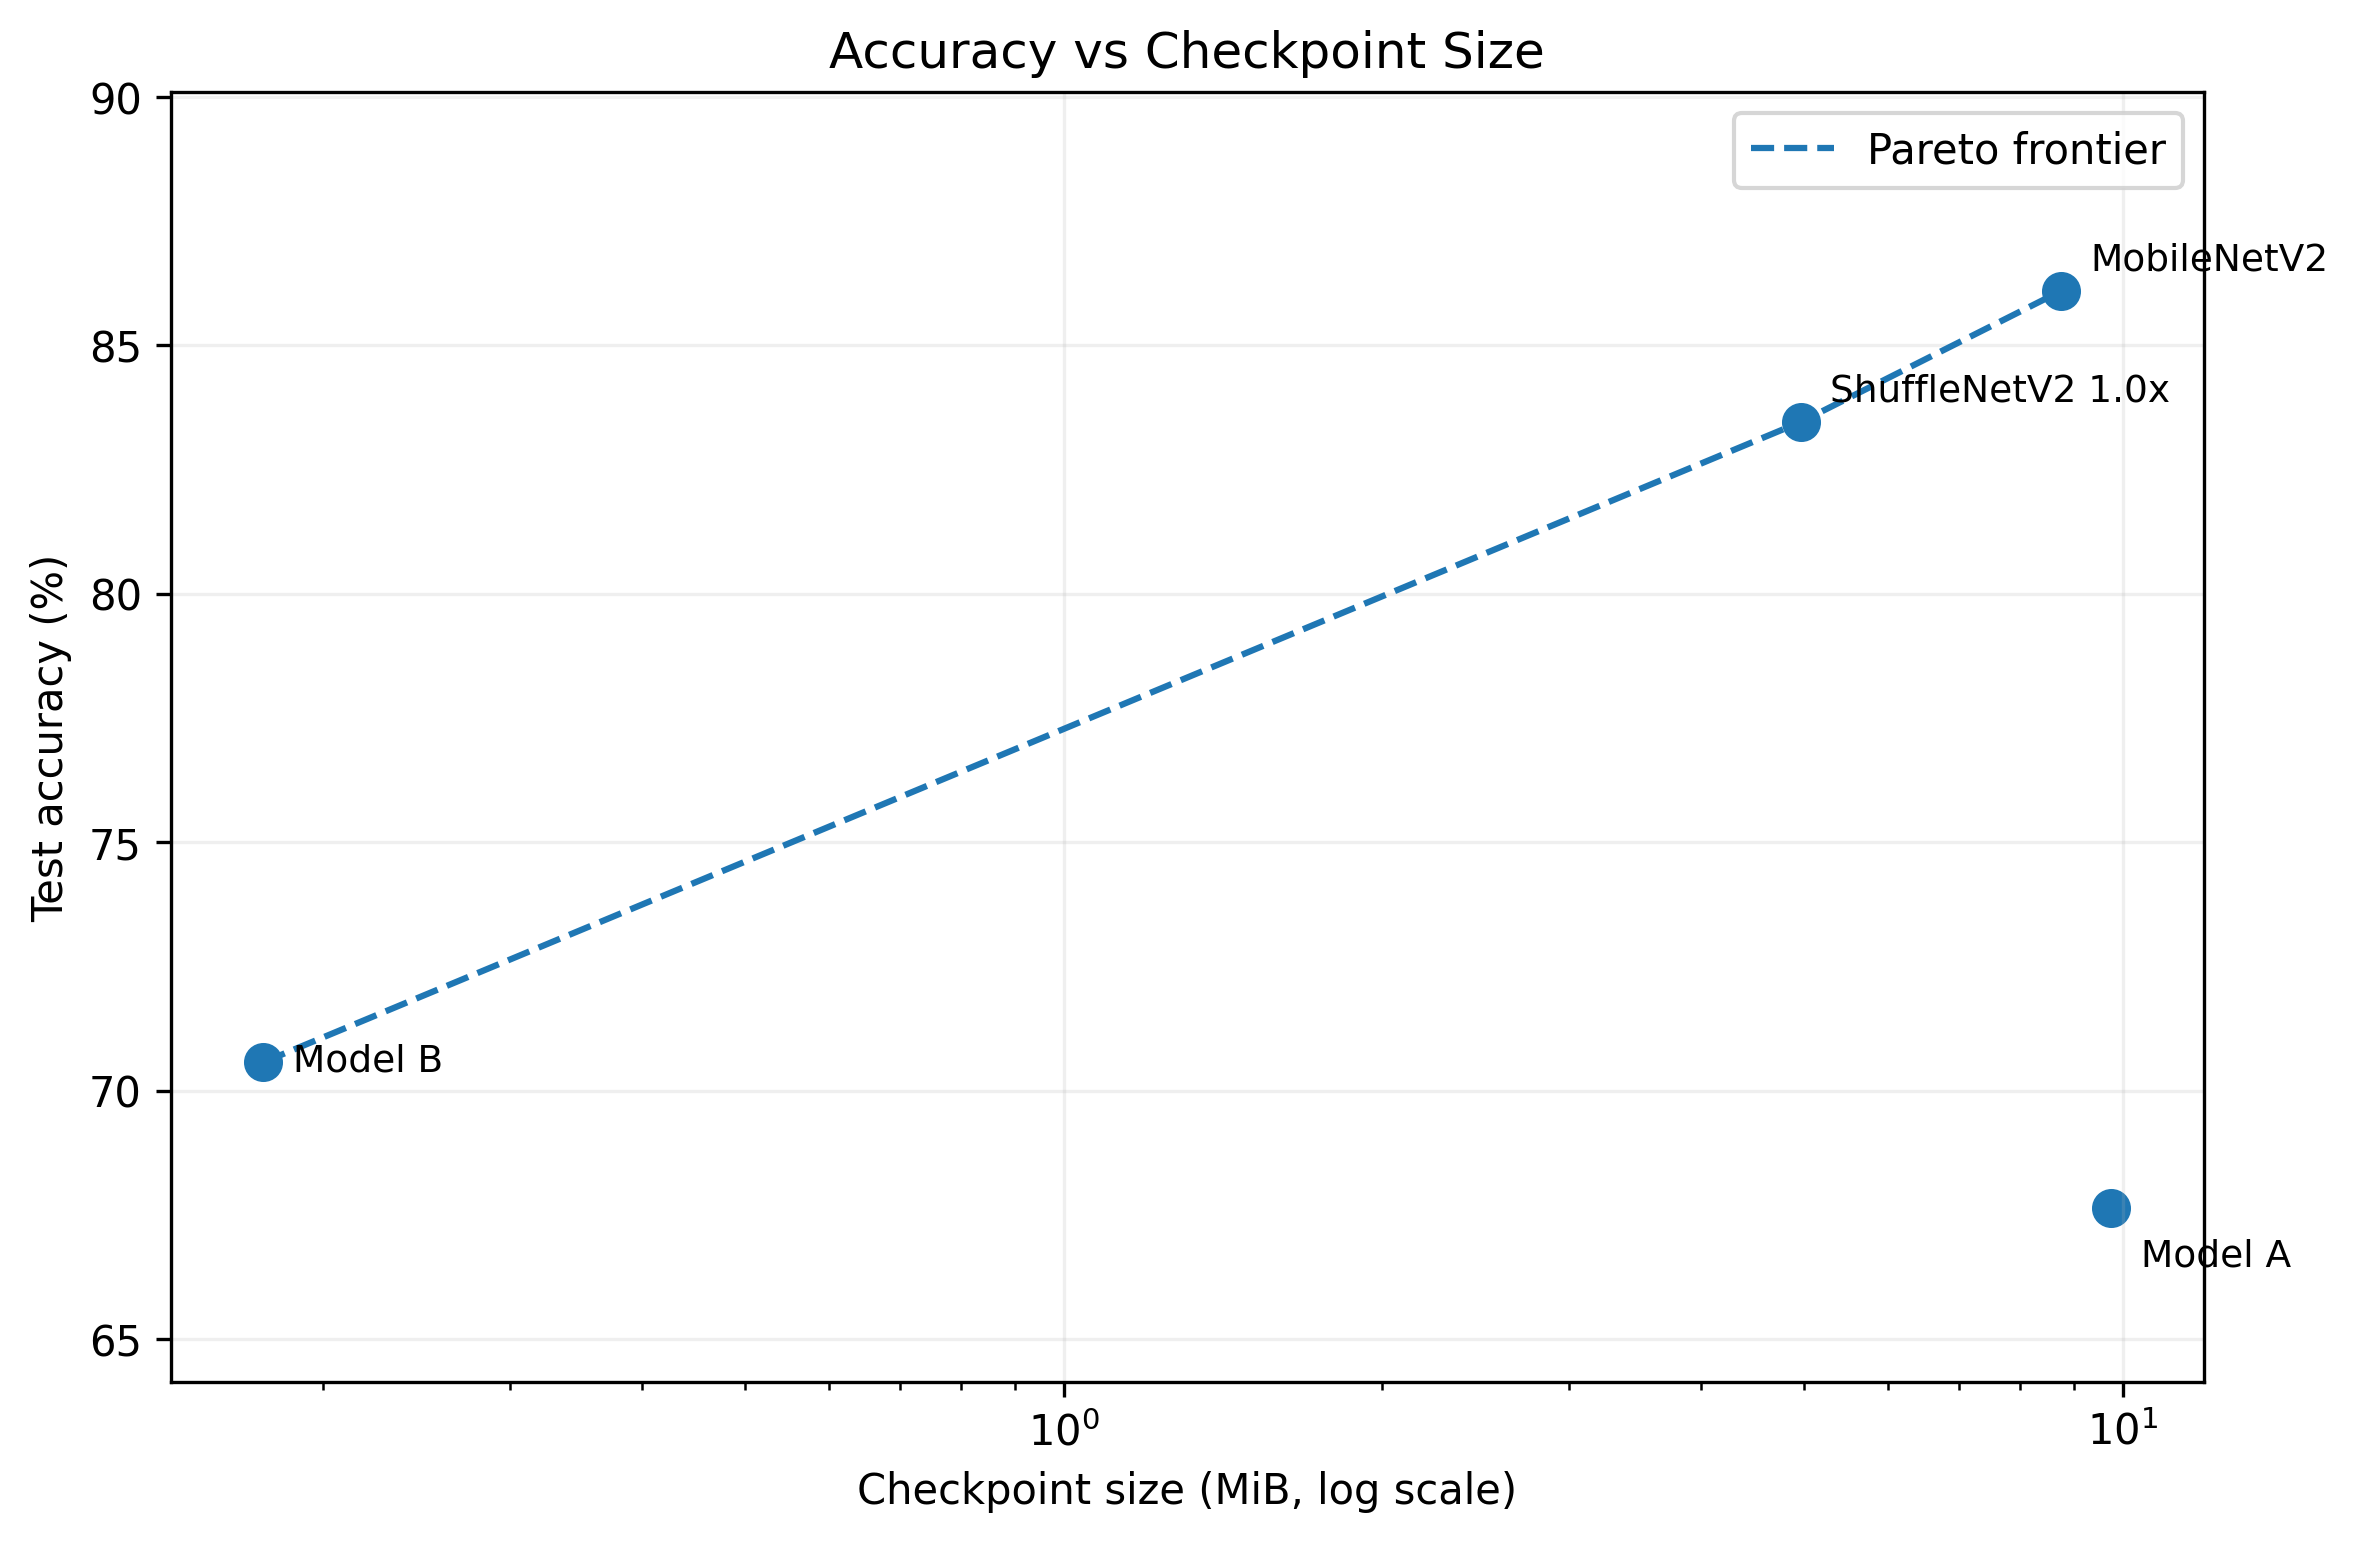
\includegraphics[width=\linewidth]{task6/accuracy_vs_model_size.png}
\caption{Accuracy versus checkpoint size.}
\end{subfigure}\hfill
\begin{subfigure}{0.49\linewidth}\centering
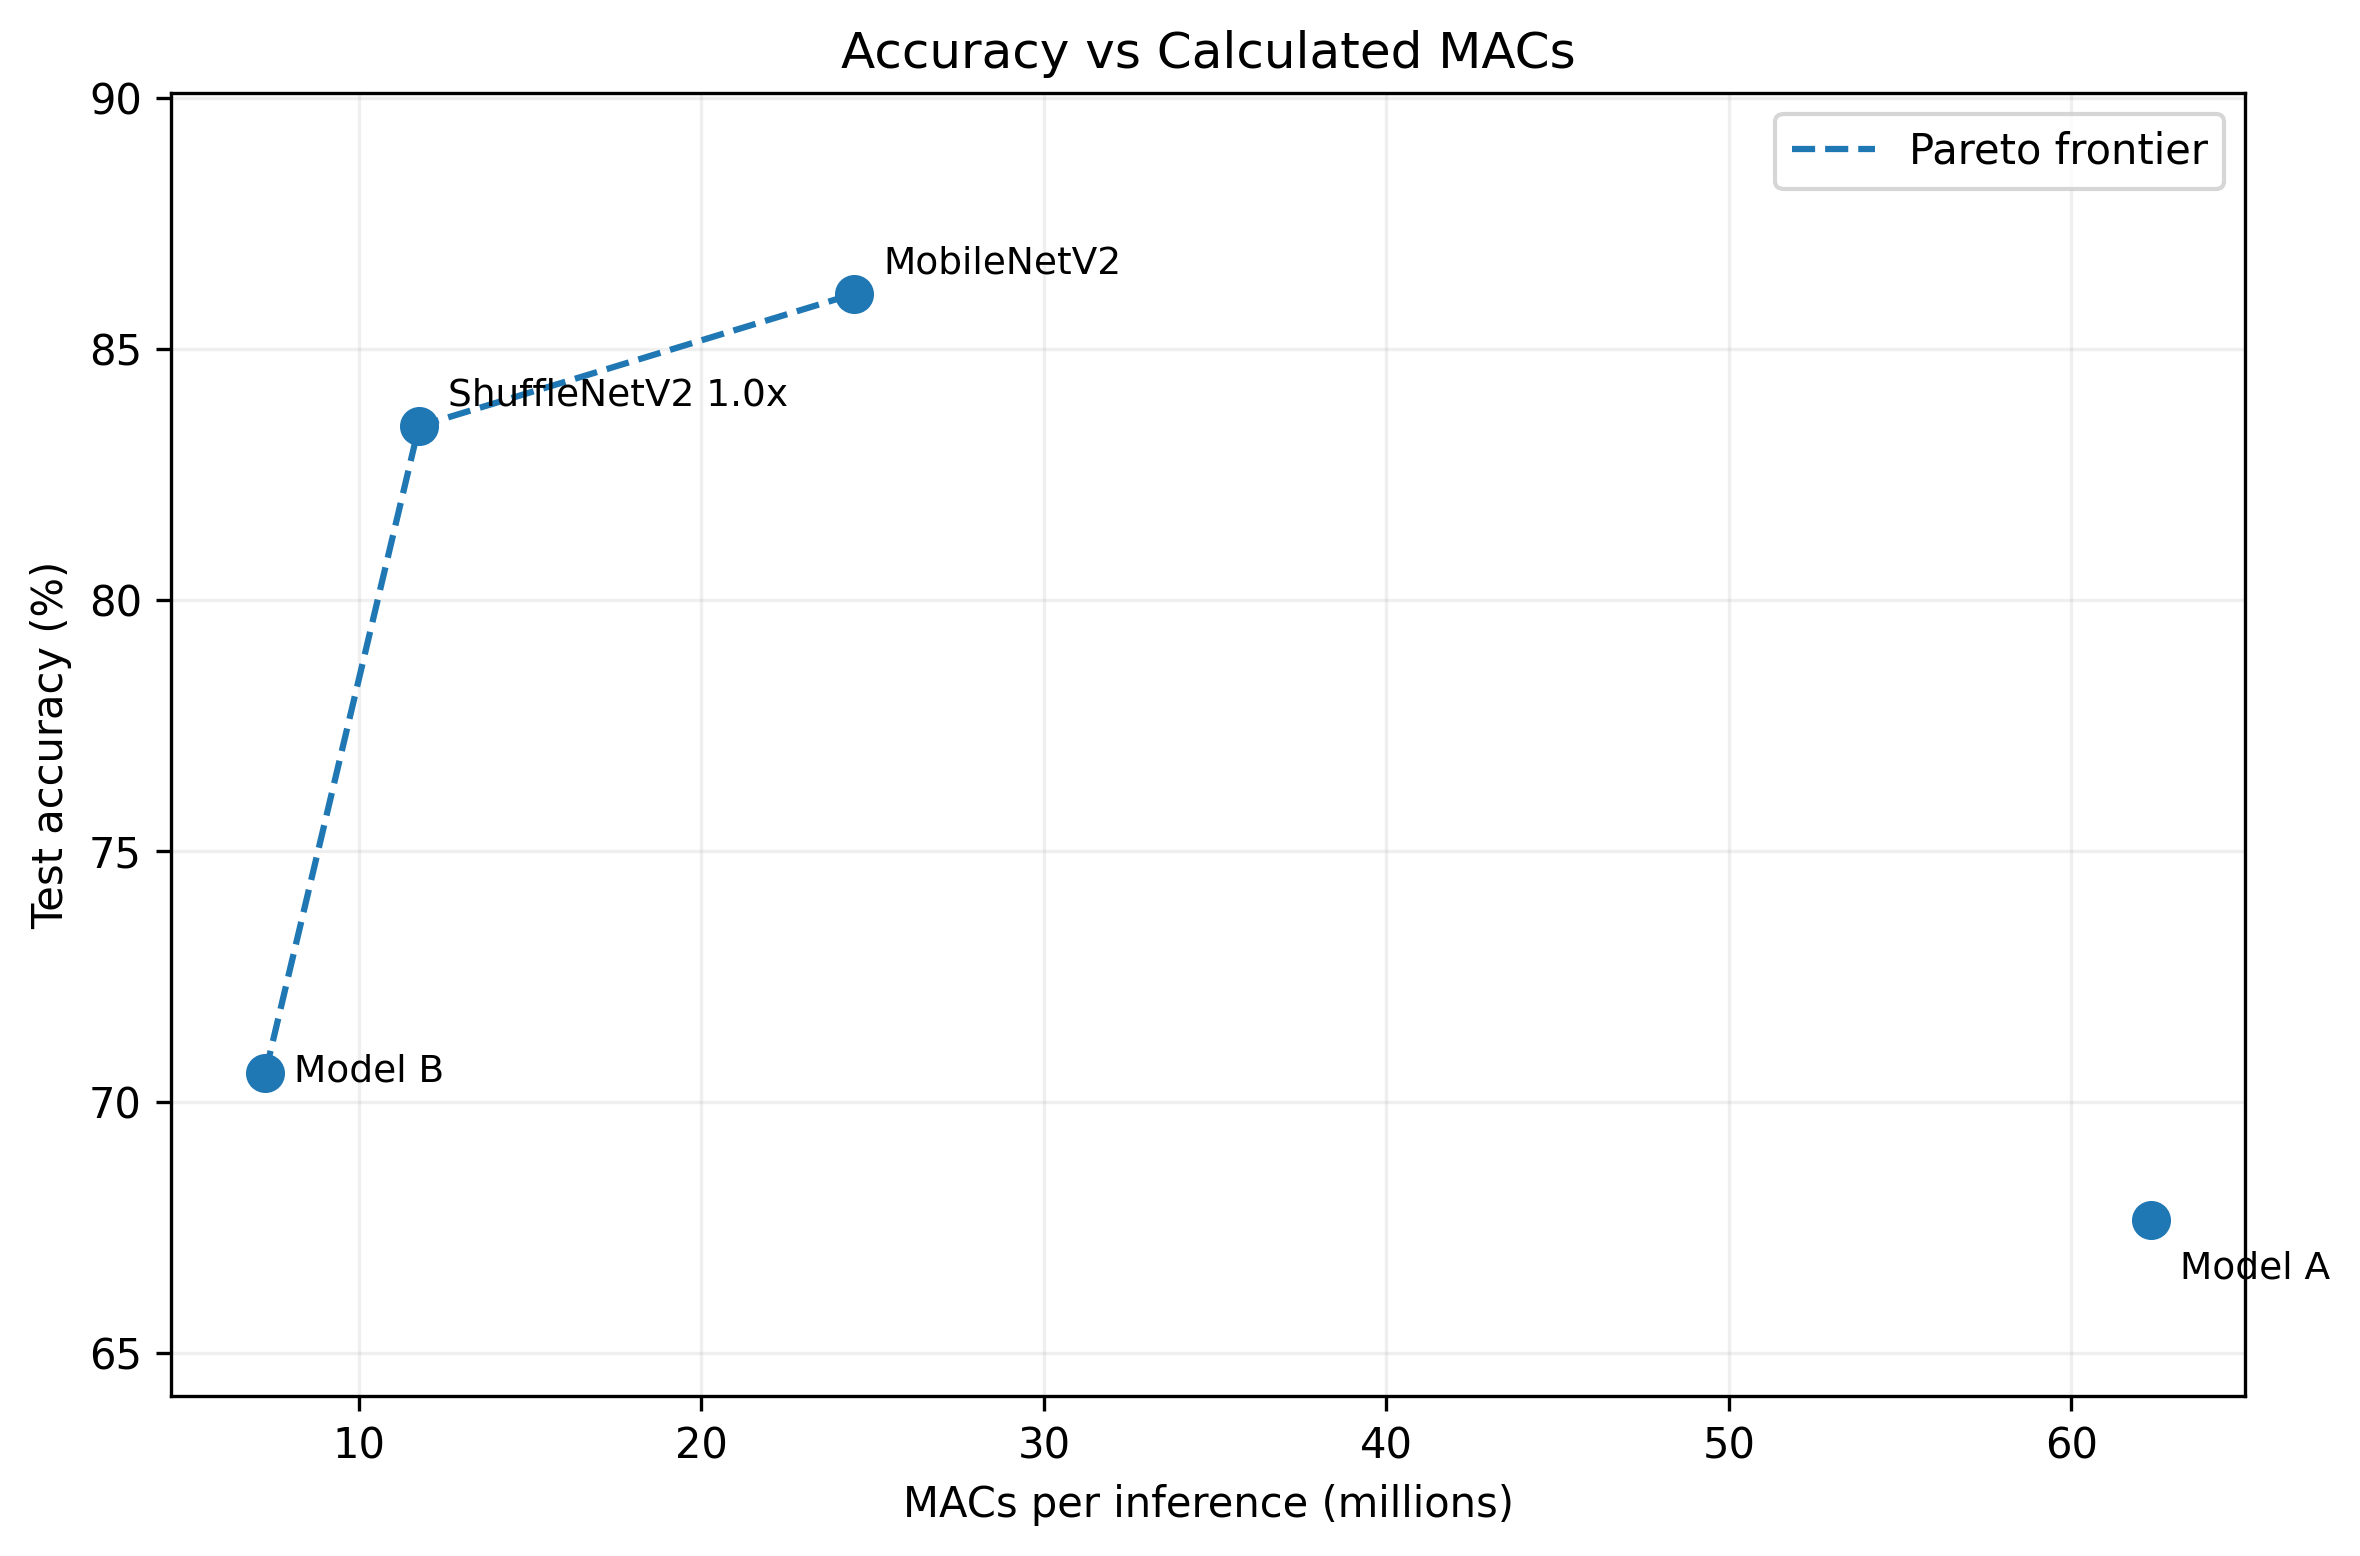
\includegraphics[width=\linewidth]{task6/accuracy_vs_macs.png}
\caption{Accuracy versus MACs.}
\end{subfigure}
\caption{Corrected accuracy-efficiency trade-offs. Model A is dominated by Model B; the remaining three models provide distinct resource/accuracy operating points.}
\end{figure}

\subsection{Engineering recommendations}
\begin{itemize}[leftmargin=*]
\item \textbf{Strictest parameter, storage, or arithmetic budget: Model B.} It is trained from scratch, contains only \ModelBParams{} parameters, and has the smallest checkpoint and MAC count. Quantization, peak-RAM profiling, operator support, and on-device latency must still be measured.
\item \textbf{Balanced accuracy and resource cost: ShuffleNetV2 1.0x.} It reaches \ShuffleAccuracy\% accuracy with substantially fewer parameters, checkpoint storage, and MACs than MobileNetV2.
\item \textbf{Accuracy-first choice: MobileNetV2.} It reaches \MobileAccuracy\% accuracy and macro F1 \MobileFOne, the strongest measured classification result, with the highest compute cost among the three final candidates.
\end{itemize}

\section{Conclusion}
On the leakage-free split, Model B outperforms the much larger conventional Model A while using \ModelBParamReductionVsA\% fewer parameters and \ModelBMACReductionVsA\% fewer MACs. MobileNetV2 and ShuffleNetV2 produce considerably higher classification performance, but their advantage accompanies greater capacity, different architectures, and ImageNet pre-training. The correct engineering choice depends on the real storage, RAM, latency, energy, and accuracy constraints; this work measures checkpoint storage and training time and calculates MACs, but does not claim unmeasured MCU RAM or latency.

\section*{Reproducibility and Submission Reminder}
All seven experiments use the same package SHA-256 and manifest SHA-256 recorded in their JSON metadata. Every history contains 20 epochs, every confusion matrix totals \DatasetTest, and cross-split duplicate content equals zero. Canonical artifacts are under \texttt{results\_clean\_split/}; the older \texttt{results/} tree is historical only.

The assignment's dataset information sheet is external to this GitHub repository. The group must update and submit that external sheet separately; this report does not claim it has been completed.

\begin{thebibliography}{9}
\bibitem{defungi} UCI Machine Learning Repository, \textit{DeFungi}, Dataset 773. \url{https://archive.ics.uci.edu/dataset/773/defungi}.
\bibitem{mobilenetv2} M. Sandler et al., ``MobileNetV2: Inverted Residuals and Linear Bottlenecks,'' \textit{CVPR}, 2018.
\bibitem{shufflenetv2} N. Ma et al., ``ShuffleNet V2: Practical Guidelines for Efficient CNN Architecture Design,'' \textit{ECCV}, 2018.
\bibitem{adam} D. P. Kingma and J. Ba, ``Adam: A Method for Stochastic Optimization,'' \textit{ICLR}, 2015.
\bibitem{pytorch} PyTorch and Torchvision model implementations, \url{https://pytorch.org/vision/stable/models.html}.
\end{thebibliography}

\end{document}
